\documentclass[english, aspectratio=169]{beamer}
% english is for the language used in standard texts (figures, tables etc)
% aspectratio of 16:9 or set it for more old school to 4:3 (without the ':')

% ---------------------------------------------------------------------------- %
% Load base preamble
% ---------------------------------------------------------------------------- %
\usepackage{import}
\subimport{./preamble/}{beamer.tex}

\usetikzlibrary{fadings}

\usepackage{multirow}

\metroset{sectionpage=none}

% ---------------------------------------------------------------------------- %
% Local settings
% ---------------------------------------------------------------------------- %
% https://tex.stackexchange.com/a/20613
\newcommand\hcancel[2][black]{\setbox0=\hbox{$#2$}%
  \rlap{\raisebox{.35\ht0}{\textcolor{#1}{\rule{\wd0}{1pt}}}}#2}

\newcommand{\B}[0]{\ensuremath{\mathbb{B}}}

\newcommand{\scan}[1]{\text{scan}(#1)}
\newcommand{\sort}[1]{\text{sort}(#1)}

\newcommand{\triple}[3]{\ensuremath{(#1, #2, #3)}}
\renewcommand{\arc}[3]{\ensuremath{#1 \xrightarrow{_{#2}} #3}}

% Horizontal legends: https://tex.stackexchange.com/a/101578
% argument #1: any options
\makeatletter
\newenvironment{customlegend}[1][]{%
    \begingroup
    % inits/clears the lists (which might be populated from previous
    % axes):
    \pgfplots@init@cleared@structures
    \pgfplotsset{#1}%
}{%
    % draws the legend:
    \pgfplots@createlegend
    \endgroup
}%

% makes \addlegendimage available (typically only available within an
% axis environment):
\def\addlegendimage{\pgfplots@addlegendimage}
\makeatother

% difficulty-level in upper right on slides:
\newcommand{\easy}[0]{\faStar[regular]}
\newcommand{\medium}[0]{\faStarHalf*}
\newcommand{\hard}[0]{\faStar[solid]}

% plot styles

\colorlet{adiar}{red}
\colorlet{buddy}{blue!40!purple}

\tikzstyle{plot_adiar}=[color=adiar, mark=diamond*, mark size=2pt, line width=1pt,
                        mark options={color=adiar, fill=adiar, opacity=0.6}]
\tikzstyle{plot_buddy}=[color=buddy, mark=pentagon*, mark size=2pt, line width=1pt,
                        mark options={color=buddy, fill=buddy, opacity=0.6}]

\tikzstyle{dots_buddy}=[color=buddy, mark=pentagon*, mark size=2pt, only marks,
                        mark options={color=buddy, fill=buddy, opacity=0.6}]
\tikzstyle{x_buddy}=[color=buddy, mark=x, mark size=2pt, only marks,
                     mark options={color=buddy, fill=buddy, opacity=0.6}]

% ------------------------------------------------------------------------------
% TITLEPAGE
% ------------------------------------------------------------------------------
\title{
  I/O-efficient Symbolic Model Checking
  \\
  {\normalsize Steffan Christ S{\o}lvsten}
}

\author{Steffan Christ S{\o}lvsten}

\institute{\includegraphics[width=0.2\linewidth]{external/aulogo_uk_var2_black.eps}}

\date{15\textsuperscript{th} of May 2025}
\begin{document}

% ---------------------------------------------------------------------------- %
\titleframe

% ---------------------------------------------------------------------------- %
% Opening Statement:
% - I/O analogy

% I would like to start with the question: what does the verb "to defer" mean?
% Luckily, I got this "Concise" English Dictionary. So, let us look up the
% meaning of this word. <...>
%
% Ah, here it is, this verb means “to put off; to postpone”.
%
% Now, this took a long time. If I had to remembered the meaning of this word
% in my "internal memory" [point at head] rather than this "external memory"
% [point at book], I could have answered this word instantly. On the bright
% side, if you need the definition of any word between default and deficiency,
% I have now found the page and can provide it to you instantly.
%
% The memory in your computer is quite similar: it has a several types of
% memory, some of which are short-term but fast [point at head] whereas others
% can store data for the long term but is very slow to access [point at book].
\begin{frame}
  \LARGE
  \begin{columns}
    \centering

    \begin{column}{0.7\textwidth}
      \begin{itemize}
      \item[\bf defer] (dif\oe'). \pause
        \emph{v.t.} to put off; to postpone.
        % \emph{v.i.} to delay; to procrastinate
        [\dots]

        % \item[\bf defer] (dif\oe').
        %   \emph{v.i.} to yield to the opinion of another.
        %   [\dots]
      \end{itemize}
    \end{column}
  \end{columns}
\end{frame}

% ---------------------------------------------------------------------------- %
% Chapter 1:
% - Motivation for critical systems
% - Systems -> Models -> Model Checking
% - State Space Explosion -> Symbolic Model Checking
%   - Relational Product
% - Binary Decision Diagram
%   - Conventional Algorithms
%   - I/O Issues

% Its memory is just one of many ways in which our modern electronics are
% extremely complicated. Yet, we depend on them every day as part of (1) our
% vehicles, (2) our hospital, and (3) our personal machines. So, it is vital
% that these actually work as intended!
\begin{frame}
  \pause

  \begin{center}
    \fontsize{42}{50}\selectfont

    \faBus* \qquad \faStethoscope \qquad \faLaptop
  \end{center}
\end{frame}

% In particular, if we consider a mere traffic light it should behave as shown
% in this diagram which we call a "transition system". In reality, a traffic
% light is much more complicated; some set of consecutive states are going to
% be "red" and so on.
%
% So, a simple property we may like to prove is that "it is either red and/or
% yellow or it is exclusively green". That is, it is not red and green at the
% same time. More complicated properties might be which colours are followed by
% which and within how much time.
%
% We can get the machine to check whether the traffic light satisfies this
% formula. To do so, it will merely check the entire state space by brute
% force. But, in more complicated systems, this transition system would be
% enormous - easily larger than the number of particles in the universe! So,
% just naively going through every possible state is not possible.
%
% Instead, we can use formulas like this one to describe a "set of states".
% Such a description can be much much smaller than the actual set of states! To
% then reason about the transitions between the states, we also use formulas
% that describe this relation. For example, if it is "red and yellow" now, then
% it will be "exclusively green" in the next state. Here, you'll notice we use
% new variables to denote the next set of states as denoted with the
% apostrophes.
\begin{frame}
  \begin{center}
    \only<1-6>{
      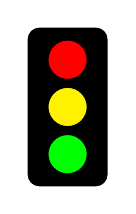
\begin{tikzpicture}
        % red
        \draw[fill=black, rounded corners] (0,0) rectangle ++(1,2);


        \draw[fill=gray!90!red]    (0.5,1.6) circle (0.25);
        \onslide<1-2,5-> {
          \draw[fill=red]          (0.5,1.6) circle (0.25);
        }

        \draw[fill=gray!90!yellow] (0.5,1.0) circle (0.25);
        \onslide<2,4> {
          \draw[fill=yellow]       (0.5,1.0) circle (0.25);
        }

        \draw[fill=gray!90!green]  (0.5,0.4) circle (0.25);
        \onslide<3,6> {
          \draw[fill=green]        (0.5,0.4) circle (0.25);
        }
      \end{tikzpicture}
    }%
    \only<7>{
      {\Large
        ``\emph{It is either red and/or ($\vee$) yellow or it is exclusively ($\oplus$) green.}''}\\
      \vspace{10pt}
      {\LARGE
        $(\mathtt{red} \lor \mathtt{yellow}) \oplus \mathtt{green}$}
    }%
    \only<8>{
      {\Large
        ``\emph{When red and yellow, it turns exclusively green.}''}\\
      \vspace{11.25pt}
      {\LARGE
        $\mathtt{red} \land \mathtt{yellow} \rightarrow \neg \mathtt{red}' \land \neg \mathtt{yellow}' \land \mathtt{green}'$}
    }%
    \only<7->{
      \vspace{11pt}
    }
  \end{center}

  \begin{figure}
    \centering

    % Fig 1.1
    \begin{tikzpicture}[scale=1.3]
      \node[shape=rectangle, thick, draw=black] at ( 0, 0)
      (r) {\texttt{red}};

      \coordinate[above=of r] (r_anchor);

      \node[shape=rectangle, thick, draw=black, right=of r]
      (ry) {\texttt{red, yellow}};

      \node[shape=rectangle, thick, draw=black, right=of ry]
      (g) {\texttt{green}};

      \node[shape=rectangle, thick, draw=black, right=of g]
      (y) {\texttt{yellow}};

      \coordinate[above=of y] (y_anchor);

      \draw[->, thick]
        (-1,0) edge (r)
        (r)    edge (ry)
        (ry)   edge (g)
        (g)    edge (y)
        (y) -- (y_anchor) -- (r_anchor) -- (r)
      ;
      \only<8>{
        \draw[very thick, dashed, ->] (ry) edge (g);
      }
    \end{tikzpicture}
  \end{figure}
\end{frame}

% These formulas can be combined to obtain the next set of states as follows:
%
% - First, we intersect the current set of states (cyan) with the relation. So,
%   now we only have restricted ourselves to the transitions that are currently
%   available; that is, the edges between the cyan and orange states.
%
% - Second, we use existential quantification to forget about where we came
%   from. So, now we only have the next set of states. But, they are still
%   marked as being next set of states.
%
% - Finally, we rename all the next set of states to current set of states.
%   At which point we can start over again to take another step in the
%   transition system
%
% The important thing is, we can explore all states of a transition system only
% using formulas, if we can use the "and", "exists, and "substitution" operators.
\begin{frame}
  \LARGE
  \begin{equation*}
    \mathit{RelProd}(S_{\vec{x}}, T_{\vec{x}, \vec{x}'}) \triangleq
    (\exists \vec{x}\ .\ S_{\vec{x}} \land T_{\vec{x}, \vec{x}'})[\vec{x}' \mapsto \vec{x}]
  \end{equation*}

  \begin{center}
    \begin{tikzpicture}
      \node[shape=rectangle, thick, draw=black] (s1) {\phantom{S}};
      \node[shape=rectangle, thick, draw=black, right=of s1] (s2) {\phantom{S}};
      \node[shape=rectangle, thick, draw=black, right=of s2] (s3) {\phantom{S}};
      \node[shape=rectangle, thick, draw=black, above=of s1] (s4) {\phantom{S}};
      \node[shape=rectangle, thick, draw=black, right=of s4] (s5) {\phantom{S}};
      \node[shape=rectangle, thick, draw=black, right=of s5] (s6) {\phantom{S}};

      \only<2-3>{
        \node[shape=rectangle, thick, fill=cyan, draw=black] {\phantom{S}};
        \node[shape=rectangle, thick, fill=cyan, draw=black, right=of s1] {\phantom{S}};
        \node[shape=rectangle, thick, fill=cyan, draw=black, above=of s1] {\phantom{S}};
      }
      \only<3-4>{
        \node[shape=rectangle, thick, pattern=checkerboard, pattern color=red, draw=black] {\phantom{S}};
        \node[shape=rectangle, thick, pattern=checkerboard, pattern color=red, draw=black, right=of s1] {\phantom{S}};
        \node[shape=rectangle, thick, pattern=checkerboard, pattern color=red, draw=black, right=of s2] {\phantom{S}};
        \node[shape=rectangle, thick, pattern=checkerboard, pattern color=red, draw=black, above=of s1] {\phantom{S}};
        \node[shape=rectangle, thick, pattern=checkerboard, pattern color=red, draw=black, right=of s4] {\phantom{S}};
      }
      \only<5>{
        \node[shape=rectangle, thick, fill=cyan, draw=black] {\phantom{S}};
        \node[shape=rectangle, thick, fill=cyan, draw=black, right=of s1] {\phantom{S}};
        \node[shape=rectangle, thick, fill=cyan, draw=black, right=of s2] {\phantom{S}};
        \node[shape=rectangle, thick, fill=cyan, draw=black, above=of s1] {\phantom{S}};
        \node[shape=rectangle, thick, fill=cyan, draw=black, right=of s4] {\phantom{S}};
      }

      \coordinate[above=0.5 of s4] (s4_anchor);
      \coordinate[above=0.5 of s6] (s6_anchor);

      \draw[->, thick]
        (s1) edge (s2)
        (s1) edge[bend left] (s4)
        (s2) edge (s3)
        (s2) edge (s5)
        (s3) edge[loop right] (s3)
        (s4) edge[bend left] (s1)
        (s4) edge (s5)
        (s5) edge (s6)
        (s6) edge (s3)
        (s6) -- (s6_anchor) -- (s4_anchor) -- (s4)
      ;

      \only<3>{
        \draw[->, thick, red]
          (s1) edge (s2)
          (s1) edge[bend left] (s4)
          (s2) edge (s3)
          (s2) edge (s5)
          (s4) edge[bend left] (s1)
          (s4) edge (s5)
        ;
      }
    \end{tikzpicture}
  \end{center}
\end{frame}

% So the question now is, how can we represent and compute on these formulas
% efficiently?
\blankframe

% The naive way to do so is to enumerate all possible assignments of 0 and 1 to
% each variable and whether the formula ends up being 1 too. But, as you can
% see, this "truth table" ends up enumerating all states individually. So, we
% have not gained anything by doing so.
\begin{frame}
  \begin{table}
    \centering\large

    \begin{tabular}{ccc|c|}
      \texttt{red} & \texttt{yellow} & \texttt{green} & $(\mathtt{red} \vee \mathtt{yellow}) \oplus \mathtt{green}$
      \\ \hline
      $0$       & $0$          & $0$         & $0$
      \\
      $0$       & $0$          & $1$         & $1$
      \\
      $0$       & $1$          & $0$         & $1$
      \\
      $0$       & $1$          & $1$         & $0$
      \\
      $1$       & $0$          & $0$         & $1$
      \\
      $1$       & $0$          & $1$         & $0$
      \\
      $1$       & $1$          & $0$         & $1$
      \\
      $1$       & $1$          & $1$         & $0$
    \end{tabular}
  \end{table}
\end{frame}

% Instead, we can use something called a Binary Decision Diagram! Here, each
% node in this diagram represents an if-then-else question on some variable. If
% the variable is 1, then you follow the solid line. If it is 0, you follow the
% dashed line. So for example, if it is 'red' the yellow light can be on or off
% (so we may as well skip it) but the green light is turned off.
%
% In many ways you can think of these as deterministic finite state machines.
% In fact, the algorithms to manipulate BDDs are conceptually the same as the
% product construction algorithms for automata.
\begin{frame}
  \begin{center}
    {\Large Binary Decision Diagram (BDD)}

    \vspace{20pt}
    \resizebox{0.25\textwidth}{!}{%
      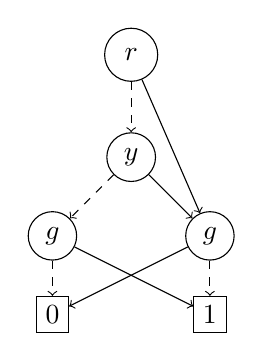
\begin{tikzpicture}
        % Fig 1.4
\node[shape=circle, draw=black, fill=white, inner sep=4.5pt] at (0, 0.3)
(r) {$r$};

\node[shape=circle, draw=black, fill=white] at ( 0, -1)
(y) {$y$};

\node[shape=circle, draw=black, fill=white] at (-1, -2)
(g1) {$g$};

\node[shape=circle, draw=black, fill=white] at ( 1, -2)
(g2) {$g$};

\node[shape=rectangle, draw=black, fill=white] at (-1,-3)
(bot) {$0$};
\node[shape=rectangle, draw=black, fill=white] at ( 1,-3)
(top) {$1$};

\draw[->, dashed]
  (r)  edge (y)
  (y)  edge (g1)
  (g1) edge (bot)
  (g2) edge (top)
;
\draw[->]
  (r)  edge (g2)
  (y)  edge (g2)
  (g1) edge (top)
  (g2) edge (bot)
;
      \end{tikzpicture}
    }
  \end{center}
\end{frame}

% Now, without going into more details, BDDs are usually implemented via
% depth-first recursion and a few hash tables. But, this means the computer has
% to constantly jump around in memory to fetch some information. Remember what
% we talked about at the beginning [point at book]? In practice, this means for
% larger BDDs, the computer is bottlenecked by the time it takes to fetch data.
%
% For example, here is an experiment I made on the BDD implementation from
% Copenhagen, named BuDDy. If we increase the size of the hash table [point to
% x-axis] such that parts of it has to be stored on the computer's disk, then
% the time it takes [point to y-axis] to run the very same set of BDD
% computations slows down by a factor of 80!
\begin{frame}
  \begin{columns}
    \begin{column}{0.38\textwidth}
      Usually BDDs are implemented by means of:
      \begin{itemize}
      \item Depth-first recursion
      \item Hash Tables
      \end{itemize}

      \vspace{50pt}
    \end{column}
    \begin{column}{0.62\textwidth}
      \centering

      \begin{tikzpicture}
        \begin{axis}[%
          width=0.9\linewidth, height=0.6\linewidth,
          every tick label/.append style={font=\scriptsize},
          % x-axis
          xlabel={Memory (GiB)},
          xmajorgrids=true,
          xmin=3.5,
          xmax=10.5,
          xtick={4, ..., 10},
          % y-axis
          ylabel={time (seconds)},
          yminorgrids=false,
          ymajorgrids=true,
          grid style={dashed,black!20},
          ]

          \draw [white, pattern=north west lines, pattern color=black!30!white]
          (axis cs: 8, 0) rectangle (axis cs: 10, 3000);

          \addplot[thick, samples=1, smooth, black, name path=barrier]
          coordinates {(8,0)(8,3000)};

          \node[black] at (axis cs: 7.4, 2800){\tiny{RAM}};
          \node[black] at (axis cs: 8.6, 2800){\tiny{Disk}};

          \addplot [style=plot_buddy]
          table {./data/cache_buddy_swap.tex};
        \end{axis}
      \end{tikzpicture}

      \qquad\qquad \texttt{BuDDy} BDD Library
    \end{column}
  \end{columns}
\end{frame}

% ---------------------------------------------------------------------------- %
% Chapter 2:
% - Areas of Research
% - Overview of Contributions (timeline)

% So right now when we try to go big, we still end up going home.
%
% The key research question for this PhD thesis is: can we compute on BDDs in
% some other way that fetches data much more nicely?
\blankframe

% This puts this research project at the intersection of three different
% disciplines in computer science.
%
% - Formal Methods is the area which is concerned with trying to prove our
%   software and hardware is correct. This provides us with the motivation and
%   use-cases.
%
% - To design the algorithms, we depend on Algorithmics that provide us with
%   the theory to design and analyse our algorithm.
%
% - And finally, we use experimental evaluation of our implementation on
%   real-life computers to further improve the design. This experimental angle
%   also uncovers new research problems to solve.
\begin{frame}
  \Large

  \begin{itemize}
  \item \textbf{Formal Methods}:

    Motivation and applications of algorithms.

  \item \textbf{Algorithmics}:

    Theoretical tools for the design and analysis of algorithms.

  \item \textbf{Algorithm Engineering}:

    Experimental evaluation and design for real-life computers.
  \end{itemize}
\end{frame}

% In particular this research project contains the following contributions
% we've made throughout the past five years:
%
% - [TOP] At the top, you can see the milestones we reached towards redesigning
%   all BDD operations. In 2021, we ironed out the foundations by tackling the
%   simplest BDD operations. At the end of 2023, we tackled quantification, and
%   finally in 2024 variable substitution. Together, this constitutes all of
%   the building blocks for the relational product we saw earlier.
%
% - [BOT] Yet, as you can see on the timeline, we our focus was initially on
%   things placed down here. These are algorithmic optimisations that
%   drastically improve performance in practice. We focused on these to make
%   sure there are no deficiencies in our algorithm which will be amplified in
%   the Quantification algorithm (and in turn the Relational Product).
%
% Up until the quantification algorithm, everything has been published at
% international conferences. The paper on Quantification is currently in
% submission. The paper on the Relational Product will the least be
% self-published on arXiv soon.
%
% On the right, there are two additional topics that are only covered in my PhD
% thesis [point to variable reordering]. Both of these have not (yet) been
% implemented. So, these contributions are only theoretical.
\begin{frame}[label=timeline]
  \begin{center}
    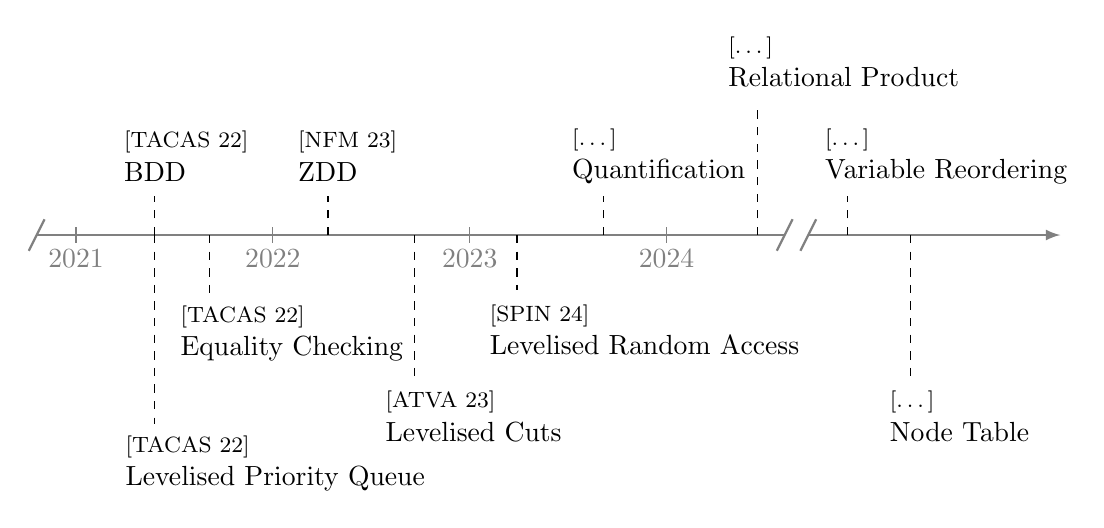
\begin{tikzpicture}
      % PhD line
\draw[gray][thick] (0.6,0.2) -- (0.4,-0.2);
\draw[gray][-, thick] (0.5,0) -- (10,0);
\draw[gray][thick] (10.1,0.2) -- (9.9,-0.2);

% 2021
\draw[gray] (1,-0.1) -- ++(0,0.2);
\node[gray] at (1,-0.3) {$2021$};

\draw[dashed, color=black] (2,0) -- ++(0,0.5);
\node[color=black, align=left] at (2.4,1.0)
{\footnotesize [TACAS 22]\\BDD};

\draw[dashed, color=black] (2,0) -- ++(0,-2.4);
\node[color=black, align=left] at (3.53,-2.9)
{\footnotesize [TACAS 22]\\Levelised Priority Queue};

\draw[dashed, color=black] (2.7,0) -- ++(0,-0.8);
\node[color=black, align=left] at (3.74,-1.25)
{\footnotesize [TACAS 22]\\Equality Checking};

% 2022
\draw[gray] (3.5,-0.1) -- ++(0,0.2);
\node[gray] at (3.5,-0.3) {$2022$};

\draw[dashed, color=black] (4.2,0) -- ++(0,0.5);
\node[color=black, align=left] at (4.45,1.0)
{\footnotesize [NFM 23]\\ZDD};

\draw[dashed, color=black] (5.3,0) -- ++(0,-1.8);
\node[color=black, align=left] at (6.05,-2.3)
{\footnotesize [ATVA 23]\\Levelised Cuts};

% 2023
\draw[gray] (6,-0.1) -- ++(0,0.2);
\node[gray] at (6,-0.3) {$2023$};

\draw[dashed, color=black] (6.6,0) -- ++(0,-0.7);
\node[color=black, align=left] at (8.22,-1.2)
{\footnotesize [SPIN 24]\\Levelised Random Access};

\draw[dashed, color=black] (7.7,0) -- ++(0,0.5);
\node[color=black, align=left] at (8.4,1.0)
{\footnotesize [\dots]\\Quantification};

% 2024
\draw[gray] (8.5,-0.1) -- ++(0,0.2);
\node[gray] at (8.5,-0.3) (y2024) {$2024$};

\draw[dashed, color=black] (9.65,0) -- ++(0,1.6);
\node[color=black, align=left] at (10.75,2.2)
{\footnotesize [\dots]\\Relational Product};

% 2025
%\draw[gray] (11,-0.1) -- ++(0,0.2);
%\node[gray] at (11,-0.3) (y2025) {$2025$};

% PostDoc (?) line
\draw[gray][thick] (10.4,0.2) -- (10.2,-0.2);
\draw[gray][-latex, thick] (10.3,0) -- (13.5,0);

% PostDoc (?)

\draw[dashed, color=black] (10.8,0) -- ++(0,0.5);
\node[color=black, align=left] at (12.05,1.0)
{\footnotesize [\dots]\\Variable Reordering};

\draw[dashed, color=black] (11.6,0) -- ++(0,-1.8);
\node[color=black, align=left] at (12.22,-2.3)
{\footnotesize [\dots]\\Node Table};

    \end{tikzpicture}
  \end{center}
\end{frame}

% So, let's take a closer look at our contributions at the top.

% ---------------------------------------------------------------------------- %
% Chapters 3, 6-7:
% - Lars Arge
% - Time-forward Processing
% - Tandem
% - Nested Tandem

% This has not been the first time that someone from Aarhus has investigated
% the efficiency with which BDD algorithms look up data in memory.
\blankframe

% Back in 1996, the late Lars Arge published paper looking at these algorithms
% I/O-complexity, which is the fancy word for this.
\begin{frame}
  \begin{center}
    {\Large\bf The I/O-Complexity of Ordered\\Binary-Decision Diagram Manipulation}

    Lars Arge

    {\footnotesize Department of Computer Science\\University of Aarhus}

    {\footnotesize August 1996}
  \end{center}
\end{frame}

% There are multiple ways one can traverse a BDD's nodes. I already mentioned
% "depth-first" which traverses its nodes according to a "last in, first out
% queue - you know them better as a stack. If you instead traverse it according
% to a "first in, first out" queue, then you end up with a breadth-first
% traversal.
%
% Arge showed that both the depth-first and breadth-first approaches are
% inefficient with respect to the numbers of lookups into the external memory.
%
% But, he also suggested an alternative: time-forward processing. Basically,
% make sure the data is sorted in some reasonable way and then use a priority
% queue to get your traversal to match a sequential reading of your data.
%
% If we go back to the analogy with the dictionary, we can process all words in
% it much faster, if we go through it one page at a time instead of randomly
% picking a word we are still missing and looking up its page.
\begin{frame}
  \Large

  Processing Order
  \begin{itemize}
  \item \textbf{Depth-first}:

    \emph{Last in, first out} Queue (Stack)

  \item \textbf{Breadth-first}:

    \emph{First in, first out} Queue

    \pause

  \item \textbf{Time-forward Processing}:

    \emph{Priority} Queue
  \end{itemize}
\end{frame}

% For BDDs, if you rearrange the picture such that you take the first level,
% then the second, and so on, then you will notice something vital: all of the
% arrows - or edges as we call them - go to the right. That is, all
% dependencies are something that will be processed *later*! Hence, we can
% *defer* the computation until we get there.
%
% In particular, since we know when we will see the dependency, we can use a
% priority queue to synchronise a list of all deferred computations with the
% order in which they are to be processed!
\begin{frame}
  \begin{columns}
    \begin{column}{0.25\textwidth}
      \centering

      \resizebox{\textwidth}{!}{%
        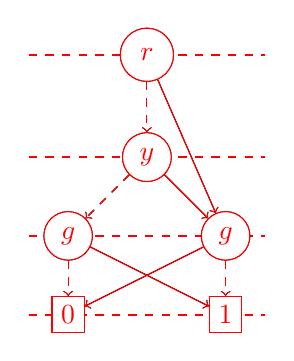
\begin{tikzpicture}
          \onslide<2>   { \draw[red, thick, dashed] (-1.5, 0.3) -- ++(3, 0); }
          \onslide<3>   { \draw[red, thick, dashed] (-1.5,-1)   -- ++(3, 0); }
          \onslide<4-5> { \draw[red, thick, dashed] (-1.5,-2)   -- ++(3, 0); }
          \onslide<6->  { \draw[red, thick, dashed] (-1.5,-3)   -- ++(3, 0); }

          % Nodes
          % Fig 1.4
\node[shape=circle, draw=black, fill=white, inner sep=4.5pt] at (0, 0.3)
(r) {$r$};

\node[shape=circle, draw=black, fill=white] at ( 0, -1)
(y) {$y$};

\node[shape=circle, draw=black, fill=white] at (-1, -2)
(g1) {$g$};

\node[shape=circle, draw=black, fill=white] at ( 1, -2)
(g2) {$g$};

\node[shape=rectangle, draw=black, fill=white] at (-1,-3)
(bot) {$0$};
\node[shape=rectangle, draw=black, fill=white] at ( 1,-3)
(top) {$1$};

\draw[->, dashed]
  (r)  edge (y)
  (y)  edge (g1)
  (g1) edge (bot)
  (g2) edge (top)
;
\draw[->]
  (r)  edge (g2)
  (y)  edge (g2)
  (g1) edge (top)
  (g2) edge (bot)
;

          % Node Highlights
          \onslide<2> {
            \node[red, shape=circle, draw=red, fill=white, inner sep=4.5pt] at (0, 0.3)
            (r) {$r$};

            \draw[red, ->, dashed] (r) edge (y);
            \draw[red, ->]         (r) edge (g2);
          }
          \onslide<3> {
            \node[red, shape=circle, draw=red, fill=white] at ( 0, -1)
            (y) {$y$};

            \draw[red, ->, dashed] (y) edge (g1);
            \draw[red, ->]         (y) edge (g2);
          }
          \onslide<4> {
            \node[red, shape=circle, draw=red, fill=white] at (-1, -2)
            (g1) {$g$};

            \draw[red, ->, dashed] (g1) edge (bot);
            \draw[red, ->]         (g1) edge (top);
          }
          \onslide<5> {
            \node[red, shape=circle, draw=red, fill=white] at ( 1, -2)
            (g2) {$g$};

            \draw[red, ->, dashed] (g2) edge (top);
            \draw[red, ->]         (g2) edge (bot);
          }
          \onslide<6> {
            \node[red, shape=rectangle, draw=red, fill=white] at (-1,-3)
            (bot) {$0$};
          }
          \onslide<7> {
            \node[red, shape=rectangle, draw=red, fill=white] at ( 1,-3)
            (top) {$1$};
          }
        \end{tikzpicture}
      }
    \end{column}
    \begin{column}{3em}
      $\implies$
    \end{column}
    \begin{column}{0.55\textwidth}
      \centering

      \resizebox{\textwidth}{!}{%
        \begin{tikzpicture}
          \node[shape=circle, draw=black, inner sep=4.5pt] at (0, 0)
          (r) {$r$};

          \node[shape=circle, draw=black] at (1, 0)
          (y) {$y$};

          \node[shape=circle, draw=black] at (2, 0)
          (g1) {$g$};

          \node[shape=circle, draw=black] at (3, 0)
          (g2) {$g$};

          \node[shape=rectangle, draw=black] at (4,0)
          (bot) {$0$};
          \node[shape=rectangle, draw=black] at (5,0)
          (top) {$1$};

          \draw[->, dashed]
            (r)  edge (y)
            (y)  edge (g1)
            (g1) edge[bend right=40] (bot)
            (g2) edge[bend left=40]  (top)
          ;
          \draw[->]
            (r)  edge[bend left=40] (g2)
            (y)  edge[bend left=40] (g2)
            (g1) edge[bend right=45] (top)
            (g2) edge (bot)
          ;

          \only<2> {
            \node[red, shape=circle, draw=red, inner sep=4.5pt] at (0, 0)
            (r) {$r$};

            \draw[red, ->, dashed] (r) edge (y);
            \draw[red, ->]         (r) edge[bend left=40] (g2);
          }
          \only<3> {
            \node[red, shape=circle, draw=red] at (1, 0)
            (y) {$y$};

            \draw[red, ->, dashed] (y) edge (g1);
            \draw[red, ->]         (y) edge[bend left=40] (g2);
          }
          \only<4> {
            \node[red, shape=circle, draw=red] at (2, 0)
            (g1) {$g$};

            \draw[red, ->, dashed] (g1) edge[bend right=40] (bot);
            \draw[red, ->]         (g1) edge[bend right=45] (top);
          }
          \only<5> {
            \node[red, shape=circle, draw=red] at (3, 0)
            (g2) {$g$};

            \draw[red, ->, dashed] (g2) edge[bend left=40]  (top);
            \draw[red, ->]         (g2) edge (bot);
          }
          \only<6> {
            \node[red, shape=rectangle, draw=red] at (4,0)
            (bot) {$0$};
          }
          \only<7> {
            \node[red, shape=rectangle, draw=red] at (5,0)
            (top) {$1$};
          }
        \end{tikzpicture}
      }
    \end{column}
  \end{columns}
\end{frame}

% And this we can use to compute the AND of two formulas represented as BDDs.
\begin{frame}[plain,noframenumbering]
  \centering\Huge $\phi \land \psi$
\end{frame}

% We'll do so in two steps: first we go over both inputs simultaneously
% top-down and construct the output. The resulting BDD can potentially be made
% smaller, which we do in the second step.
%
% Let's start with taking a slightly deeper look at the first phase.
\begin{frame}{$\phi \land \psi$}
  \only<1>{
    \setvalue{tandem_apply  = black}
    \setvalue{tandem_reduce = black}
  }
  \only<2>{
    \setvalue{tandem_apply  = black}
    \setvalue{tandem_reduce = lightgray}
  }

  \begin{center}
    \begin{tikzpicture}[scale=1.25]
      % tikz/tandem.tex (but simplified)

% Boxes
\draw[color=\getvalue{tandem_apply}, thick]
(0,0) rectangle ++(2,1)
node[pos=.5]{\large \texttt{Apply} ($\land$)}
;
\draw[color=\getvalue{tandem_reduce}, thick]
(4,0) rectangle ++(2,1)
node[pos=.5]{\large \texttt{Reduce}}
;

% Arcs
\draw[->, color=\getvalue{tandem_apply}, thick]
(-0.5,0.8) -- ++(0.5,0)
node[pos=-0.5]{\large $f$}
;
\draw[->, color=\getvalue{tandem_apply}, thick]
(-0.5,0.2) -- ++(0.5,0)
node[pos=-0.5]{\large $g$}
;

\draw[densely dashed, ->, thick] (2,0.5) -- ++(2,0)
node[pos=0.5,above]
{transposed}
node[pos=0.5,below]
{\texttt{arcs}}
;

\draw[->, color=\getvalue{tandem_reduce}, thick]
(6,0.5) -- ++(0.5,0)
node[pos=2.0]{\large $f \land g$}
;

    \end{tikzpicture}
  \end{center}
\end{frame}

% Apply Phase:
%   Without going into too many details, the Apply an And operation takes the
%   two inputs on the left and sweeps through them level by level. As we go
%   down, more and more of the output is resolved and is output on the right.
%
%   Due to the way in which the output is created, we actually have reversed
%   the edges. But, this actually is to our benefit as you'll see soon.
%
%   Because note, the output is not as small as it could. For example, the 'd'
%   node on the lower right may as well be skipped - one reaches '0' either
%   way. Similarly, the two other 'd' nodes are duplicates and can be merged
%   together.
\begin{frame}{$\phi \land \psi$}
  \begin{columns}
    \begin{column}{0.25\textwidth}
      \centering

      \begin{tikzpicture}
        % sweepline
        \onslide<2> { \draw[red, thick, dashed] (-1.5, 0)   -- ++(3, 0); }
        \onslide<3> { \draw[red, thick, dashed] (-1.5,-1.5) -- ++(3, 0); }
        \onslide<4> { \draw[red, thick, dashed] (-1.5,-3)   -- ++(3, 0); }
        \onslide<5> { \draw[red, thick, dashed] (-1.5,-4.5) -- ++(3, 0); }
        \onslide<6> { \draw[red, thick, dashed] (-1.5,-6)   -- ++(3, 0); }

        %   % nodes
  \node[shape = circle, draw = black]
  (0) {$x_0$};

  \node[shape = circle, draw = black, below right= .4cm and .5cm of 0]
  (1) {$x_1$};

  \node[shape = circle, draw = black, below left=.4cm and .5cm of 1]
  (2) {$x_2$};

  \node[shape = circle, draw = black, below left=.4cm and .5cm of 2]
  (31) {$x_3$};
  \node[shape = circle, draw = black, below right=.4cm and .5cm of 2]
  (32) {$x_3$};
  
  % leafs
  \node[shape = rectangle, draw = black, below=.4cm of 31]
  (sink_T) {$\top$};

  \node[shape = rectangle, draw = black, below=.4cm of 32]
  (sink_F) {$\bot$};

  % arcs
  \draw[->, dashed]
    (0)  edge (2)
    (1)  edge (2)
    (2)  edge (31)
    (31) edge (sink_T)
    (32) edge (sink_F)
  ;

  \draw[->]
    (0)  edge (1)
    (1)  edge (32)
    (2)  edge (32)
    (31) edge (sink_F)
    (32) edge (sink_T)
  ;

        % nodes
        \node[shape=circle, draw=black, fill=white, inner sep=4.5pt] at ( 0, 0)
        (0) {$a$};

        \node[shape=circle, draw=black, fill=white] at ( 1,-1.5)
        (1) {$b$};

        \node[shape=circle, draw=black, fill=white, inner sep=4.5pt] at ( 0,-3)
        (2) {$c$};

        \node[shape=circle, draw=black, fill=white] at (-1,-4.5)
        (31) {$d$};
        \node[shape=circle, draw=black, fill=white] at ( 1,-4.5)
        (32) {$d$};

        % leafs
        \node[shape=rectangle, draw=black, fill=white] at ( 1,-6)
        (bot) {$0$};
        \node[shape=rectangle, draw=black, fill=white] at (-1,-6)
        (top) {$1$};

        % arcs
        \draw[->, dashed]
          (0)  edge (2)
          (1)  edge (2)
          (2)  edge (31)
          (31) edge (top)
          (32) edge (bot)
        ;

        \draw[->]
          (0)  edge (1)
          (1)  edge (32)
          (2)  edge (32)
          (31) edge (bot)
          (32) edge (top)
        ;
      \end{tikzpicture}
    \end{column}
    \begin{column}{1em}
      \centering $\land$
    \end{column}
    \begin{column}{0.25\textwidth}
      \centering

      \begin{tikzpicture}
        % sweepline
        \onslide<2> { \draw[red, thick, dashed] (-1.5, 0)   -- ++(3, 0); }
        \onslide<3> { \draw[red, thick, dashed] (-1.5,-1.5) -- ++(3, 0); }
        \onslide<4> { \draw[red, thick, dashed] (-1.5,-3)   -- ++(3, 0); }
        \onslide<5> { \draw[red, thick, dashed] (-1.5,-4.5) -- ++(3, 0); }
        \onslide<6> { \draw[red, thick, dashed] (-1.5,-6)   -- ++(3, 0); }

        %   % nodes
  \node[shape = circle, draw = black]
  (0) {$x_0$};

  \node[shape = circle, draw = black, below left=1.4cm and .5cm of 0]
  (21) {$x_2$};

  \node[shape = circle, draw = black, below right=1.4cm and .5cm of 0]
  (22) {$x_2$};

  \node[shape = circle, draw = black, below right=0.4cm and .5cm of 21]
  (3) {$x_3$};

  % leafs
  \node[shape = rectangle, draw = black, below right=.4cm and .5cm of 3]
  (sink_F) {$\bot$};

  \node[shape = rectangle, draw = black, below left=.4cm and .5cm of 3]
  (sink_T) {$\top$};

  % arcs
  \draw[->, dashed]
    (0)  edge (21)
    (21) edge (sink_T)
    (22) edge (3)
    (3)  edge (sink_T)
  ;

  \draw[->]
    (0)  edge (22)
    (21) edge (3)
    (22) edge (sink_F)
    (3)  edge (sink_F)
  ;

        % nodes
        \node[shape=circle, draw=black, fill=white, inner sep=4.5pt] at ( 0, 0)
        (0) {$a$};

        \node[shape=circle, draw=black, fill=white, inner sep=4.5pt] at (-1,-3)
        (21) {$c$};

        \node[shape=circle, draw=black, fill=white, inner sep=4.5pt] at ( 1,-3)
        (22) {$c$};

        \node[shape=circle, draw=black, fill=white] at ( 0,-4.5)
        (3) {$d$};

        % leafs
        \node[shape=rectangle, draw=black, fill=white] at ( 1,-6)
        (bot) {$0$};
        \node[shape=rectangle, draw=black, fill=white] at (-1,-6)
        (top) {$1$};

        % arcs
        \draw[->, dashed]
          (0)  edge (21)
          (21) edge (top)
          (22) edge (3)
          (3)  edge (top)
        ;

        \draw[->]
          (0)  edge (22)
          (21) edge (3)
          (22) edge (bot)
          (3)  edge (bot)
        ;
      \end{tikzpicture}
    \end{column}
    \begin{column}{3em}
      \centering $\implies$
    \end{column}
    \begin{column}{0.45\textwidth}
      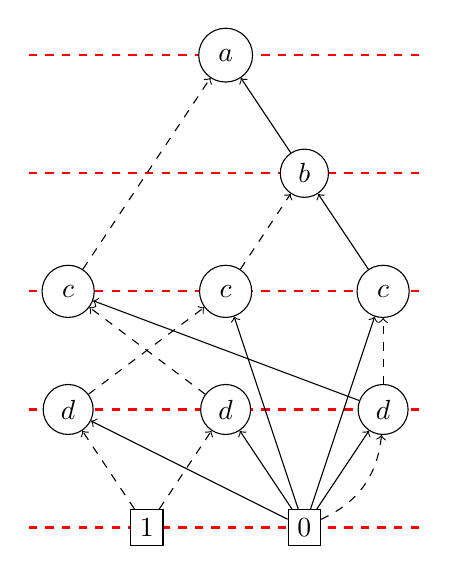
\begin{tikzpicture}
        % sweepline
        \onslide<2> { \draw[red, thick, dashed] (-2.5, 0)   -- ++(5, 0); }
        \onslide<3> { \draw[red, thick, dashed] (-2.5,-1.5) -- ++(5, 0); }
        \onslide<4> { \draw[red, thick, dashed] (-2.5,-3)   -- ++(5, 0); }
        \onslide<5> { \draw[red, thick, dashed] (-2.5,-4.5) -- ++(5, 0); }
        \onslide<6> { \draw[red, thick, dashed] (-2.5,-6)   -- ++(5, 0); }

        % levels
        \onslide<2-> {
          \node[shape=circle, draw=black, fill=white, inner sep=4.5pt] at ( 0, 0)
          (0) {$a$};
        }

        \onslide<3-> {
          \node[shape=circle, draw=black, fill=white] at ( 1,-1.5)
          (1) {$b$};

          \draw[->] (1) edge (0);
        }

        \onslide<4-> {
          \node[shape=circle, draw=black, fill=white, inner sep=4.5pt] at (-2,-3)
          (21) {$c$};
          \node[shape=circle, draw=black, fill=white, inner sep=4.5pt] at ( 0,-3)
          (22) {$c$};
          \node[shape=circle, draw=black, fill=white, inner sep=4.5pt] at ( 2,-3)
          (23) {$c$};

          \draw[->, dashed]
            (21) edge (0)
            (22) edge (1)
          ;
          \draw[->] (23) edge (1);
        }

        \onslide<5-> {
          \node[shape=circle, draw=black, fill=white] at (-2,-4.5)
          (31) {$d$};
          \node[shape=circle, draw=black, fill=white] at ( 0,-4.5)
          (32) {$d$};
          \node[shape=circle, draw=black, fill=white] at ( 2,-4.5)
          (33) {$d$};

          \draw[->, dashed]
            (31) edge (22)
            (32) edge (21)
            (33) edge (23)
          ;
          \draw[->] (33) edge (21);
        }

        \onslide<6-7> {
          \node[shape=rectangle, draw=black, fill=white] at ( 1,-6)
          (bot) {$0$};
          \node[shape=rectangle, draw=black, fill=white] at (-1,-6)
          (top) {$1$};

          \draw[->, dashed]
            (bot) edge[bend right] (33)
            (top) edge (31)
            (top) edge (32)
          ;
          \draw[->]
            (bot) edge (22)
            (bot) edge (23)
            (bot) edge (31)
            (bot) edge (32)
            (bot) edge (33)
          ;
        }
      \end{tikzpicture}
    \end{column}
  \end{columns}
\end{frame}

% This is where the second phase comes in!
\begin{frame}{$\phi \land \psi$}
  \setvalue{tandem_apply  = lightgray}
  \setvalue{tandem_reduce = black}

  \begin{center}
    \begin{tikzpicture}[scale=1.25]
      % tikz/tandem.tex (but simplified)

% Boxes
\draw[color=\getvalue{tandem_apply}, thick]
(0,0) rectangle ++(2,1)
node[pos=.5]{\large \texttt{Apply} ($\land$)}
;
\draw[color=\getvalue{tandem_reduce}, thick]
(4,0) rectangle ++(2,1)
node[pos=.5]{\large \texttt{Reduce}}
;

% Arcs
\draw[->, color=\getvalue{tandem_apply}, thick]
(-0.5,0.8) -- ++(0.5,0)
node[pos=-0.5]{\large $f$}
;
\draw[->, color=\getvalue{tandem_apply}, thick]
(-0.5,0.2) -- ++(0.5,0)
node[pos=-0.5]{\large $g$}
;

\draw[densely dashed, ->, thick] (2,0.5) -- ++(2,0)
node[pos=0.5,above]
{transposed}
node[pos=0.5,below]
{\texttt{arcs}}
;

\draw[->, color=\getvalue{tandem_reduce}, thick]
(6,0.5) -- ++(0.5,0)
node[pos=2.0]{\large $f \land g$}
;

    \end{tikzpicture}
  \end{center}
\end{frame}

% Reduce Phase:
%   I'll spare you the technical details. But, assuming everything below some
%   level already is minimized, then we can find all redundant and duplicate
%   nodes on said level relatively simply. Hence, we want to process the
%   diagram from the bottom and up. Again, we want to use time-forward
%   processing but this time to send information up. Luckily, the edges were
%   reversed, so they already match this flow!
%
%   So, we start from the bottom, and construct level by level the minimized
%   output.
\begin{frame}{$\phi \land \psi$}
  \begin{columns}
    \begin{column}{0.45\textwidth}
      \centering

      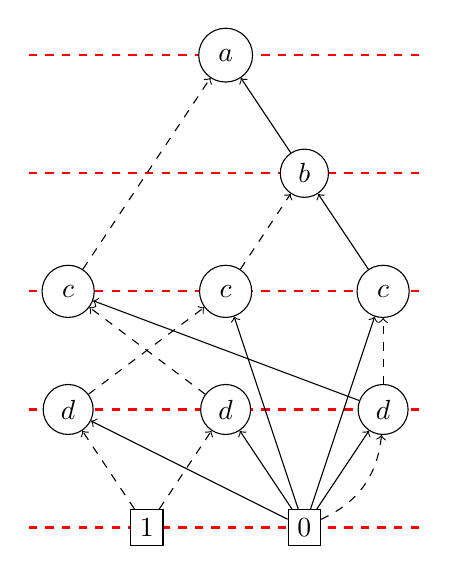
\begin{tikzpicture}
        % sweepline
        \onslide<2> { \draw[red, thick, dashed] (-2.5,-6)   -- ++(5, 0); }
        \onslide<3> { \draw[red, thick, dashed] (-2.5,-4.5) -- ++(5, 0); }
        \onslide<4> { \draw[red, thick, dashed] (-2.5,-3)   -- ++(5, 0); }
        \onslide<5> { \draw[red, thick, dashed] (-2.5,-1.5) -- ++(5, 0); }
        \onslide<6> { \draw[red, thick, dashed] (-2.5, 0)   -- ++(5, 0); }

        % nodes
        \node[shape=circle, draw=black, fill=white, inner sep=4.5pt] at ( 0, 0)
        (0) {$a$};

        \node[shape=circle, draw=black, fill=white] at ( 1,-1.5)
        (1) {$b$};

        \node[shape=circle, draw=black, fill=white, inner sep=4.5pt] at (-2,-3)
        (21) {$c$};
        \node[shape=circle, draw=black, fill=white, inner sep=4.5pt] at ( 0,-3)
        (22) {$c$};
        \node[shape=circle, draw=black, fill=white, inner sep=4.5pt] at ( 2,-3)
        (23) {$c$};


        \node[shape=circle, draw=black, fill=white] at (-2,-4.5)
        (31) {$d$};
        \node[shape=circle, draw=black, fill=white] at ( 0,-4.5)
        (32) {$d$};
        \node[shape=circle, draw=black, fill=white] at ( 2,-4.5)
        (33) {$d$};

        \node[shape=rectangle, draw=black, fill=white] at ( 1,-6)
        (bot) {$0$};
        \node[shape=rectangle, draw=black, fill=white] at (-1,-6)
        (top) {$1$};

        % arcs
        \draw[->, dashed]
          (21) edge (0)
          (22) edge (1)
          (31) edge (22)
          (32) edge (21)
          (33) edge (23)
          (bot) edge[bend right] (33)
          (top) edge (31)
          (top) edge (32)
        ;
        \draw[->]
          (1) edge (0)
          (23) edge (1)
          (33) edge (21)
          (bot) edge (22)
          (bot) edge (23)
          (bot) edge (31)
          (bot) edge (32)
          (bot) edge (33)
        ;
      \end{tikzpicture}
    \end{column}
    \begin{column}{3em}
      \centering $\implies$
    \end{column}
    \begin{column}{0.3\textwidth}
      \centering

      \begin{tikzpicture}
        % sweepline
        \onslide<2> { \draw[red, thick, dashed] (-1.5,-6)   -- ++(3, 0); }
        \onslide<3> { \draw[red, thick, dashed] (-1.5,-4.5) -- ++(3, 0); }
        \onslide<4> { \draw[red, thick, dashed] (-1.5,-3)   -- ++(3, 0); }
        \onslide<5> { \draw[red, thick, dashed] (-1.5,-1.5) -- ++(3, 0); }
        \onslide<6> { \draw[red, thick, dashed] (-1.5, 0)   -- ++(3, 0); }

        %   % nodes
  \node[shape = circle, draw = black]
  (0) {$x_0$};

  \node[shape = circle, draw = black, below right= .4cm and .5cm of 0]
  (1) {$x_1$};

  \node[shape = circle, draw = black, below left=.4cm and .5cm of 1]
  (2) {$x_2$};

  \node[shape = circle, draw = black, below left=.4cm and .5cm of 2]
  (31) {$x_3$};
  \node[shape = circle, draw = black, below right=.4cm and .5cm of 2]
  (32) {$x_3$};
  
  % leafs
  \node[shape = rectangle, draw = black, below=.4cm of 31]
  (sink_T) {$\top$};

  \node[shape = rectangle, draw = black, below=.4cm of 32]
  (sink_F) {$\bot$};

  % arcs
  \draw[->, dashed]
    (0)  edge (2)
    (1)  edge (2)
    (2)  edge (31)
    (31) edge (sink_T)
    (32) edge (sink_F)
  ;

  \draw[->]
    (0)  edge (1)
    (1)  edge (32)
    (2)  edge (32)
    (31) edge (sink_F)
    (32) edge (sink_T)
  ;

        % leafs
        \onslide<2-> {
          \node[shape=rectangle, draw=black, fill=white] at ( 1,-6)
          (bot) {$0$};
          \node[shape=rectangle, draw=black, fill=white] at (-1,-6)
          (top) {$1$};
        }

        % nodes
        \onslide<3-> {
          \node[shape=circle, draw=black, fill=white] at ( 0,-4.5)
          (3) {$d$};

          \draw[->, dashed] (3) edge (top);
          \draw[->]         (3) edge (bot);
        }

        \onslide<4-> {
          \node[shape=circle, draw=black, fill=white, inner sep=4.5pt] at ( 0,-3)
          (2) {$c$};

          \draw[->, dashed] (2) edge (3);
          \draw[->]         (2) edge (bot);
        }

        \onslide<5-> {
          \node[shape=circle, draw=black, fill=white] at ( 1,-1.5)
          (1) {$b$};

          \draw[->, dashed] (1) edge (2);
          \draw[->]         (1) edge (bot);
        }

        \onslide<6-7> {
          \node[shape=circle, draw=black, fill=white, inner sep=4.5pt] at ( 0, 0)
          (0) {$a$};

          \draw[->, dashed] (0) edge (2);
          \draw[->]         (0) edge (1);
        }
      \end{tikzpicture}
    \end{column}
  \end{columns}
\end{frame}

% If we look at its theoretical running time, the depth-first version uses
% linear time with respect to the input and the output size. The time-forward
% processing is almost the same but with an additional log-factor. Yet, our
% version is I/O-efficient.
%
% That is, we do a little bit more computations to drastically improve the
% memory accesses.
%
% Around at this point is where Lars Arge's contributions back in 1995 ends; we
% simplified and improved upon his original design before going to the more
% complex operations.
\begin{frame}{$\phi \land \psi$}
  \centering

  {\Large Depth-first}\\\vspace{5pt}
  {\LARGE $\Oh{N+T}$}\\
  {\emph{but not I/O efficient!}}

  \vspace{20pt}

  {\Large Time-forward Processing}\\\vspace{5pt}
  {\LARGE $\Oh{(N+T) \log (N+T)}$}\\
  {\emph{but I/O efficient!}}

  \vspace{20pt}

  {\large $N$: Input Size \qquad $T$: (Unreduced) Output Size}

\end{frame}

% So, the second operation we needed was the existential quantification.
%
%   For a single variable, this is quite easy: whether there exists a value for
%   'x' to make the formula evaluate to '1' is the same as asking whether the
%   formula with '0' or '1' put in the place of 'x' makes it so.
%
%   We can compute this using the algorithm I just showed you. We can also use
%   it to quantify multiple variables one-by-one. Yet doing them one-by-one
%   seems like a lot of work - we would like an algorithm that takes care of
%   all variables at once.
\begin{frame}[plain,noframenumbering]
  \centering\Huge $\exists x: \phi(x)$\onslide<2>{ $\equiv$ $\phi(0) \lor \phi(1)$}
\end{frame}

% To do so, we build on top of the previous algorithms as follows:
%
%   First, we transpose the graph. That is, we reverse the edges.
%
%   With the edges reversed, we can forward information up rather than down.
%   This allows us to accumulate the result from the bottom up in the *outer*
%   Reduce sweep.
%
%   In particular, we accumulates the result of multiple *nested* Apply-Reduce
%   cycles. Each cycle applies a single Or-operation to a to be quantified
%   variable.
\begin{frame}{$\exists \vec{x} : \phi(\vec{x})$}
  \only<1>{
    \setvalue{tandem_transpose = black}
    \setvalue{tandem_outer     = black}
    \setvalue{tandem_inner     = black}
  }
  \only<2>{
    \setvalue{tandem_transpose = black}
    \setvalue{tandem_outer     = lightgray}
    \setvalue{tandem_inner     = lightgray}
  }
  \only<3>{
    \setvalue{tandem_transpose = lightgray}
    \setvalue{tandem_outer     = black}
    \setvalue{tandem_inner     = lightgray}
  }
  \only<4>{
    \setvalue{tandem_transpose = lightgray}
    \setvalue{tandem_outer     = lightgray}
    \setvalue{tandem_inner     = black}
  }

  \begin{center}
    \begin{tikzpicture}[scale=1.25]
      % Boxes (outer)
\draw[thick, color=\getvalue{tandem_transpose}] (0,0) rectangle ++(2,1)
node[pos=.5]{\large \texttt{Transpose}};

\draw[thick, color=\getvalue{tandem_outer}] (3.5,0) rectangle ++(2,1)
node[pos=.5]{\large \texttt{Reduce}};

% Arcs (outer)
\draw[->, thick, color=\getvalue{tandem_transpose}] (-0.5,0.5) -- ++(0.5,0)
node[pos=-0.35]{\large $f$};

\draw[->, thick, color=\getvalue{tandem_transpose}, dashed] (2,0.8) -- ++(1.5,0);

\draw[->, thick, color=\getvalue{tandem_outer}] ( 3.0,0.2) -- ++(0.5,0)
node[pos=-0.35]{\large $\vec{x}$};

\draw[->, thick, color=\getvalue{tandem_outer}] (5.5,0.5) -- ++(3,0)
node[pos=1.3]{\large $\exists \vec{x}.\ f(\vec{x})$};

% Boxes (inner)
\draw[thick, color=\getvalue{tandem_inner}] (6.5,-2) rectangle ++(2,1)
node[pos=.5]{\large \texttt{Apply} ($\lor$)};
\draw[thick, color=\getvalue{tandem_inner}] (3.5,-2) rectangle ++(2,1)
node[pos=.5]{\large \texttt{Reduce}};

% Arcs (inner)
\draw[->, thick, color=\getvalue{tandem_outer}] (7.5,0.5) -- ++(0,-1.5);

\draw[->, thick, color=\getvalue{tandem_inner}, dashed] (6.5,-1.5) -- ++(-1.0,0);

\draw[->, thick, color=\getvalue{tandem_inner}] (4.5,-1) -- ++(0,1);

    \end{tikzpicture}
  \end{center}
\end{frame}

% If we take a deeper look, it looks like this:
%   In this example, we want to quantify variables 'b' and 'd'.
%
% Transposition:
%   On the left we have the already transposed diagram.
%
% Outer Reduce:
%   We start out as with the other Reduce by creating the output from the
%   bottom up. But, we pause after being done with processing level 'd' since
%   that is one of the variables we wanted to quantify.
%
% Inner Apply-Reduce:
%   The edges are pointing downwards on the output. So, we can use that
%   immediately as the input for another sweep where we compute the Or of both
%   outgoing options for the 'd' node.
%
%   While doing so, we remember which nodes from the original input on the left
%   is connected to the new temporary nodes in the middle.
%
%   Now, we have another graph with reversed edges. We can construct the new
%   output anew by reducing this one superimposed on the original input!
%
% Outer Reduce:
%   And we keep going until we reach the level of variable 'b' which we also
%   want to quantify in this example.
%
% Inner Apply-Reduce:
%   And, again we go down to create the diagram whether either option on the
%   'b' node could reach the '1'. And, we reduce the temporary diagram in the
%   middle superimposed on the original input on the left ...
%
% Outer Reduce:
%   ... until we have reduced the entire thing and are done.
\begin{frame}{$\exists \vec{x} : \phi(\vec{x}) \qquad \vec{x} = \{ b, d \}$}
  \begin{columns}
    \begin{column}[b]{0.3\textwidth}
      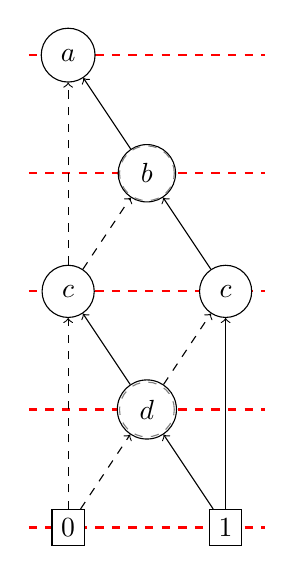
\begin{tikzpicture}
        % sweepline
        \onslide<2>    { \draw[red, thick, dashed] (-1.5,-6)   -- ++(3, 0); }
        \onslide<3-7>  { \draw[red, thick, dashed] (-1.5,-4.5) -- ++(3, 0); }
        \onslide<8>    { \draw[red, thick, dashed] (-1.5,-3)   -- ++(3, 0); }
        \onslide<9-15> { \draw[red, thick, dashed] (-1.5,-1.5) -- ++(3, 0); }
        \onslide<16>   { \draw[red, thick, dashed] (-1.5, 0)   -- ++(3, 0); }

        % nodes
        \node[shape=rectangle, draw=black, fill=white] at (-1,-6)
        (bot) {$0$};
        \node[shape=rectangle, draw=black, fill=white] at ( 1,-6)
        (top) {$1$};
        \node[shape=circle, draw=black, fill=white, inner sep=4.5pt] at ( 0,-4.5)
        (d) {$d$};
        \node[shape=circle, draw=gray, dashed, inner sep=7pt] at ( 0,-4.5) {};
        \node[shape=circle, draw=black, fill=white, inner sep=4.5pt] at (-1,-3)
        (c1) {$c$};
        \node[shape=circle, draw=black, fill=white, inner sep=4.5pt] at ( 1,-3)
        (c2) {$c$};
        \node[shape=circle, draw=black, fill=white, inner sep=4.5pt] at ( 0,-1.5)
        (b) {$b$};
        \node[shape=circle, draw=gray, dashed, inner sep=7pt] at ( 0,-1.5) {};
        \node[shape=circle, draw=black, fill=white, inner sep=4.5pt] at (-1, 0)
        (a) {$a$};

        % arcs
        \draw[->, dashed]
          (bot) edge (d)
          (bot) edge (c1)
          (d)   edge (c2)
          (c1)  edge (b)
          (c1)  edge (a)
        ;
        \draw[->]
          (top) edge (d)
          (top) edge (c2)
          (d)   edge (c1)
          (c2)  edge (b)
          (b)   edge (a)
        ;
      \end{tikzpicture}
    \end{column}
    \begin{column}[b]{0.3\textwidth}
      % nested sweep : 'd'
      \only<4-9> {
        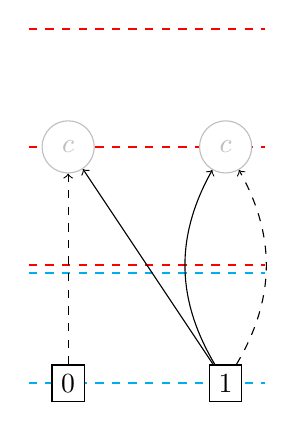
\begin{tikzpicture}
          % sweepline
          \onslide<5-6> { \draw[cyan, thick, dashed] (-1.5,-6)   -- ++(3, 0); }
          \onslide<3-7> { \draw[red,  thick, dashed] (-1.5,-4.5) -- ++(3, 0); }
          \onslide<4,7> { \draw[cyan, thick, dashed] (-1.5,-4.6) -- ++(3, 0); }
          \onslide<8>   { \draw[red, thick, dashed] (-1.5,-3)   -- ++(3, 0); }
          \onslide<9>   { \draw[red,  thick, dashed] (-1.5,-1.5) -- ++(3, 0); }

          \onslide<5-> {
            % nodes
            \node[shape=rectangle, draw=black, fill=white] at (-1,-6)
            (bot) {$0$};
            \node[shape=rectangle, draw=black, fill=white] at ( 1,-6)
            (top) {$1$};

            \node[shape=circle, draw=lightgray, fill=white, inner sep=4.5pt] at (-1,-3)
            (c1) {\color{lightgray} $c$};
            \node[shape=circle, draw=lightgray, fill=white, inner sep=4.5pt] at ( 1,-3)
            (c2) {\color{lightgray} $c$};

            % arcs
            \draw[->, dashed]
              (bot) edge (c1)
              (top) edge[bend right] (c2)
            ;
            \draw[->]
              (top) edge (c1)
              (top) edge[bend left] (c2)
            ;
          }
        \end{tikzpicture}
      }%
      \only<10-16> {
        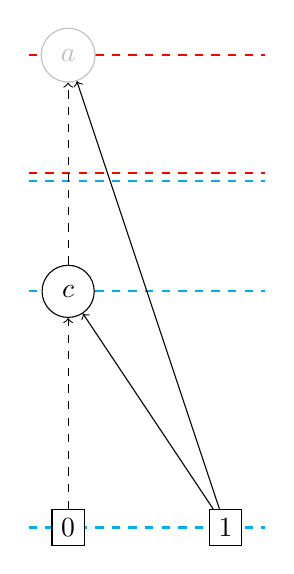
\begin{tikzpicture}
          % sweepline
          \onslide<12-13> { \draw[cyan, thick, dashed] (-1.5,-6)   -- ++(3, 0); }
          \onslide<11,14> { \draw[cyan, thick, dashed] (-1.5,-3)   -- ++(3, 0); }
          \onslide<10,15> { \draw[cyan, thick, dashed] (-1.5,-1.6) -- ++(3, 0); }
          \onslide<10-15> { \draw[red,  thick, dashed] (-1.5,-1.5) -- ++(3, 0); }
          \onslide<16>  { \draw[red, thick, dashed] (-1.5, 0)   -- ++(3, 0); }

          % nodes
          \onslide<11-> {
            \node[shape=circle, draw=lightgray, fill=white, inner sep=4.5pt] at (-1, 0)
            (a) {\color{lightgray} $a$};
            \node[shape=circle, draw=black, fill=white, inner sep=4.5pt] at (-1,-3)
            (c1) {$c$};

            \draw[->, dashed] (c1)  edge (a);
          }
          \onslide<12-> {
            \node[shape=rectangle, draw=black, fill=white] at (-1,-6)
            (bot) {$0$};
            \node[shape=rectangle, draw=black, fill=white] at ( 1,-6)
            (top) {$1$};

            \draw[->, dashed] (bot) edge (c1);
            \draw[->]
              (top) edge (c1)
              (top) edge (a)
            ;
          }
        \end{tikzpicture}
      }
    \end{column}
    \begin{column}[b]{3em}
      \centering $\implies$

      \vspace{85pt}
    \end{column}
    \begin{column}[b]{0.3\textwidth}
      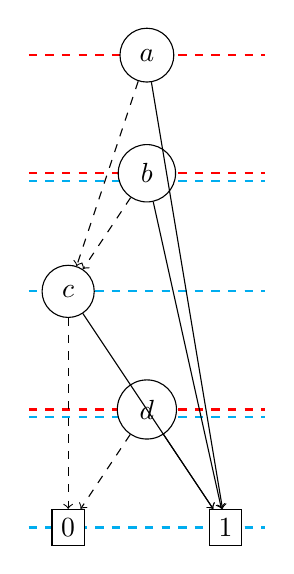
\begin{tikzpicture}
        % sweepline(s)
        \onslide<2>         { \draw[red,  thick, dashed] (-1.5,-6)   -- ++(3, 0); }
        \onslide<5-6,12-13> { \draw[cyan, thick, dashed] (-1.5,-6)   -- ++(3, 0); }
        \onslide<3-7>       { \draw[red,  thick, dashed] (-1.5,-4.5) -- ++(3, 0); }
        \onslide<4,7>       { \draw[cyan, thick, dashed] (-1.5,-4.6) -- ++(3, 0); }
        \onslide<8>         { \draw[red,  thick, dashed] (-1.5,-3)   -- ++(3, 0); }
        \onslide<11,14>     { \draw[cyan, thick, dashed] (-1.5,-3)   -- ++(3, 0); }
        \onslide<9-15>      { \draw[red,  thick, dashed] (-1.5,-1.5) -- ++(3, 0); }
        \onslide<10,15>     { \draw[cyan, thick, dashed] (-1.5,-1.6) -- ++(3, 0); }
        \onslide<16>        { \draw[red, thick, dashed] (-1.5, 0)   -- ++(3, 0); }

        % output
        \onslide<2-> {
          \node[shape=rectangle, draw=black, fill=white] at (-1,-6)
          (bot) {$0$};
          \node[shape=rectangle, draw=black, fill=white] at ( 1,-6)
          (top) {$1$};
        }

        \onslide<3-5> {
          \node[shape=circle, draw=black, fill=white, inner sep=4.5pt] at ( 0,-4.5)
          (d) {$d$};

          \draw[->, dashed] (d) edge (bot);
          \draw[->]         (d) edge (top);
        }

        \onslide<8-12,14-> {
          \node[shape=circle, draw=black, fill=white, inner sep=4.5pt] at (-1,-3)
          (c1) {$c$};

          \draw[->, dashed] (c1) edge (bot);
          \draw[->]         (c1) edge (top);
        }

        \onslide<9-12> {
          \node[shape=circle, draw=black, fill=white, inner sep=4.5pt] at ( 0,-1.5)
          (b) {$b$};

          \draw[->, dashed] (b) edge (c1);
          \draw[->]         (b) edge (top);
        }

        \onslide<16-17> {
          \node[shape=circle, draw=black, fill=white, inner sep=4.5pt] at ( 0, 0)
          (a) {$a$};

          % arcs
          \draw[->, dashed] (a) edge (c1);
          \draw[->]         (a) edge (top);
        }
      \end{tikzpicture}
    \end{column}
  \end{columns}
\end{frame}

% This more complex algorithm does not improve on the theoretical worst-case
% running time. But, that also seems unlikely if not impossible. Yet, we
% improve the running time in practice by almost a factor of two.
\begin{frame}{$\exists \vec{x} : \phi(\vec{x})$}
  \centering

  {\Large Single Variable Quantification}\\\vspace{5pt}
  {\LARGE $\Oh{N^{2^k} \log(N^{2^k})}$}\\

  \vspace{20pt}

  {\Large Nested Sweeping}\\\vspace{5pt}
  {\LARGE $\Oh{N^{2^k} \log(N^{2^k})}$}\\
  {\emph{but $1.8 \times$ faster!}}

  \vspace{20pt}

  {\large $N$: Input Size}
\end{frame}

% The last operation we needed was variable substitution. That is, we need to
% rename variables.
\begin{frame}[plain,noframenumbering]
  \centering\Huge $[x \mapsto y]$
\end{frame}

% What we notice is, that for our use-case we only really care about *monotone*
% variable substitutions. These are substitutions that do not change the order
% of the variables: a variable 'x_i' that precedes another 'x_j' also precedes
% it after renaming.
%
% The important thing is, that such substitutions do not affect the shape of
% the binary decision diagram. For example, by renaming 'c' to 'b', we do not
% have to move its node on this diagram on the other side of the node with
% variable 'a'.
%
% The offshoot of this is that variable substitution can be done by literally
% just copy-pasting the diagram and renaming the variables within its nodes.
% Furthermore, we can also incorporate the renaming for free inside of the other
% algorithms I showed you earlier.
\begin{frame}[t]{$[x \mapsto y]$}
  \begin{definition}
    A relabelling $\pi$ is monotone if $x_i < x_j \implies \pi(x_i) < \pi(x_j)$.
  \end{definition}
  \begin{lemma}
    If $\pi$ is monotone, then the BDD $f(\vec{x})$ is isomorphic to $f(\pi(\vec{x}))$.
  \end{lemma}

  \bigskip

  \only<1> {
    \begin{columns}
      \begin{column}{0.25\textwidth}
        \centering

        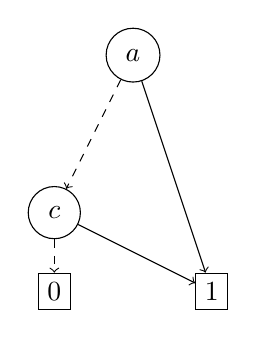
\begin{tikzpicture}
          % nodes
          \node[shape=rectangle, draw=black, fill=white] at (-1,-3)
          (bot) {$0$};
          \node[shape=rectangle, draw=black, fill=white] at ( 1,-3)
          (top) {$1$};
          \node[shape=circle, draw=black, fill=white, inner sep=4.5pt] at (-1,-2)
          (c) {$c$};
          \node[shape=circle, draw=black, fill=white, inner sep=4.5pt] at ( 0, 0)
          (a) {$a$};

          % arcs
          \draw[->, dashed]
          (a) edge (c)
          (c) edge (bot)
          ;
          \draw[->]
          (a) edge (top)
          (c) edge (top)
          ;
        \end{tikzpicture}
      \end{column}
      \begin{column}{3em}
        \centering $\implies$
      \end{column}
      \begin{column}{0.25\textwidth}
        \centering

        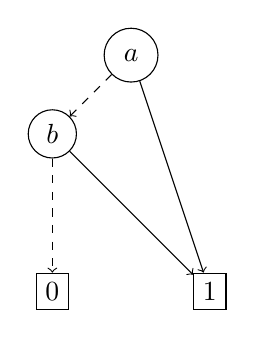
\begin{tikzpicture}
          % nodes
          \node[shape=rectangle, draw=black, fill=white] at (-1,-3)
          (bot) {$0$};
          \node[shape=rectangle, draw=black, fill=white] at ( 1,-3)
          (top) {$1$};
          \node[shape=circle, draw=black, fill=white] at (-1,-1)
          (b) {$b$};
          \node[shape=circle, draw=black, fill=white, inner sep=4.5pt] at ( 0, 0)
          (a) {$a$};

          % arcs
          \draw[->, dashed]
          (a) edge (b)
          (b) edge (bot)
          ;
          \draw[->]
          (a) edge (top)
          (b) edge (top)
          ;
        \end{tikzpicture}
      \end{column}
    \end{columns}
  }%
  \only<2> {
    \begin{itemize}
    \item {\bf One can apply $\pi$ in a single linear scan.}

      $\Oh{N}$ time, $2 \cdot \scan{N}$ I/Os, and $N$ external space.

    \item {\bf One can incorporate $\pi$ into a (succeeding) top-down \texttt{Apply} sweep.}

      $\Oh{N}$ time, $0$ I/Os, and $0$ external space.

    \item {\bf One can incorporate $\pi$ into a (preceeding) bottom-up \texttt{Reduce} sweep.}

      $\Oh{n}$ time, $0$ I/Os, and $0$ external space.
    \end{itemize}
  }
\end{frame}

% As I showed for the And operation, these time-forward procession algorithms
% are in theory faster than the conventional depth-first algorithms when memory
% accesses are the bottleneck. So, what about in practice?
%
% To answer this question, we have implemented these algorithms in C++ to
% create a new BDD library called Adiar.
%
% So, how well do we do...?
\blankframe
\begin{frame}[plain,noframenumbering]{}
  \vspace{60pt}

  \begin{center}
    {\fontsize{42}{50}\selectfont \texttt{Adiar}\textsuperscript{\normalsize 1}}

    \rule{180pt}{0.6pt}

    {
      \href{http://github.com/ssoelvsten/adiar}{github.com/ssoelvsten/adiar}
    }
  \end{center}

  \vspace{40pt}

  \textcolor{gray}{
    \rule{150pt}{0.6pt}
  }\\
  \textcolor{gray}{\footnotesize \textsuperscript{1}
    adiar $\langle$ portugese $\rangle$ (verb) : to defer, to postpone.
  }
\end{frame}

% Let us start with a slightly simpler application than the Relational Product.
% In a Quantified Boolean Formula we alternate between Exists and Forall
% quantifications of variables in some formula. Among other things, this can be
% used to encode 2-player games; if we can find an assignment to the
% existential variables that solves the equation then we have a strategy for
% one of the players to be guaranteed a win in the game.
%
% On this plot you can see on the x-axis how much time our implementation needs
% to compute on each formula. On the y-axis, we have how much faster or slower
% the BuDDy implementation from Copenhagen is. If the dot is above the 1x line,
% then we are faster.
%
% This picture shows the general pattern we've seen in our experiments:
%   On the left-most third we have the very small instances. Here, we are much
%   much slower because our implementation has not been build with them in
%   mind. But, that was not really our goal.
%
%   Then in the middle third, we have the medium instances where the difference
%   between the algorithms flattens. In these cases, our algorithms have picked
%   up their pace. As we can see here, using our implementation is only at the
%   cost of being about 4 times slower.
%
%   And finally, on the last third we have the large instances. Here, the
%   conventional implementation gets close to its memory limit and slows down.
%   For the last two instances marked with crosses, it wasn't even able to
%   solve them as it hit the boundaries of internal memory!
%
% Now, this experiment was done with as much internal memory as possible. This
% is mainly to the benefit of the conventional algorithms, since they can
% survive for as long as possible. That is, these experimental results gives
% you a good idea as to how well our algorithm does in the worst possible case.
\begin{frame}[t]
  \begin{center}
    \Large
    Quantified Boolean Formul{\ae} (QBF) of 2-player games:\\
    {$\exists \vec{x} \forall \vec{y} \dots \exists \vec{z} : \phi(\vec{x}, \vec{y}, \dots, \vec{z}) \stackrel{?}{=} 1$}
  \end{center}

  \begin{center}
    \begin{tikzpicture}
      \begin{axis}[%
        width=0.8\linewidth, height=0.42\linewidth,
        every tick label/.append style={font=\scriptsize},
        % x-axis
        xlabel={\small \texttt{Adiar} Running Time (s)},
        xmin=0.01,
        xmax=10000,
        xtick={0.01,0.1,1,10,100,1000,10000},
        xmode=log,
        % y-axis
        ylabel={\small \texttt{BuDDy} Relative Running Time},
        ymin=0.00390625,
        ymax=5.0,
        ytick = {0.00390625,0.015625,0.0625,0.25,1,4},
        yticklabels = {
          $2^{-8} \times$,
          $2^{-6} \times$,
          $2^{-4} \times$,
          $2^{-2} \times$,
          $1 \times$,
          $2^{2} \times$
        },
        ymode=log,
        % grid
        grid style={dashed,black!12},
        ]

        % 1 line
        \addplot[domain=0.001:100000, samples=8, color=black]
        {1};

        % vertical 1s line
        \draw[densely dotted, opacity=0.4] (0,1.0) -- (0,-5.0);
        % vertical 100s line
        \draw[densely dotted, opacity=0.4] (4.6,1.0) -- (4.6,-5.0);

        % data (solved)
        \addplot+ [forget plot, style=dots_buddy, mark size=5pt]
        table {./data/qbf.buddy.solved.tex};

        % data (timeouts)
        \addplot+ [forget plot, style=x_buddy, mark size=4pt]
        table {./data/qbf.buddy.timeouts.tex};
      \end{axis}
    \end{tikzpicture}
  \end{center}
\end{frame}

% So, what happens if we decrease the amount of memory? In particular, let's
% take a look at the running time of the relational product in three different
% real-world transition systems.
%
% On the x-axis you have the amount of internal memory available whereas on the
% y-axis you have the time needed for our implementation, Adiar, and
% also BuDDy from Copenhagen.
%
% - First of all, you can see that the running time of our algorithm is
%   pretty much completely independent of the amount of internal memory. It's
%   actually quite eery, if I may say so.
%
% - BuDDy on the other hand, begins to slow down quite considerably as we
%   begin to decrease the amount of memory. In the two examples on the left, it
%   stops working when we get below about 4 GiB of memory. On the one on the
%   right, it does not crash but slows down by several orders of magnitude!
\begin{frame}[t]
  \begin{center}
    \Large
    Relational Product in a Transition System:\\
    $\mathit{RelProd}(S_{\vec{x}}, T_{\vec{x}, \vec{x}'}) \triangleq
    (\exists \vec{x}\ .\ S_{\vec{x}} \land T_{\vec{x}, \vec{x}'})[\vec{x}' \mapsto \vec{x}]$
  \end{center}

  \begin{figure}
    \centering

    \begin{subfigure}{0.3\linewidth}
      \centering

      \qquad\quad{\tiny \texttt{GPUForwardProgress}~20a}

      \begin{tikzpicture}
        \begin{axis}[%
          width=1.05\linewidth, height=1\linewidth,
          every tick label/.append style={font=\scriptsize},
          % x-axis
          xlabel={\scriptsize Memory (GiB)},
          xmin=0.8,
          xtick={1,2,4,8},
          xticklabels={1,2,4,8},
          xmax=10,
          xmode=log,
          % y-axis
          ylabel={\scriptsize Running Time (s)},
          ymin=100,
          ymax=43200,
          ytick={100,1000,10000,100000},
          ymode=log,
          % grid
          grid style={dashed,black!12},
          ]

          % BuDDy memory out
          % \addplot+ [style=x_buddy, forget plot] coordinates {
          % (2, 36000)
          % };

          %   data
          \addplot+ [style=plot_adiar]
          table {./data/memory.gpufp_20_a.adiar.tex};

          \addplot+ [style=plot_buddy]
          table {./data/memory.gpufp_20_a.buddy.tex};
        \end{axis}
      \end{tikzpicture}

    \end{subfigure}
    \hspace{-30pt}
    \begin{subfigure}{0.3\linewidth}
      \centering

      \quad{\tiny \texttt{SmartHome}~16}

      \begin{tikzpicture}
        \begin{axis}[%
          width=1.05\linewidth, height=1\linewidth,
          every tick label/.append style={font=\scriptsize},
          % x-axis
          xlabel={\scriptsize Memory (GiB)},
          xmin=0.8,
          xtick={1,2,4,8},
          xticklabels={1,2,4,8},
          xmax=10,
          xmode=log,
          % y-axis
          ymin=100,
          ymax=43200,
          ytick={100,1000,10000,100000},
          yticklabels={,,,},
          ymode=log,
          % grid
          grid style={dashed,black!12},
          ]

          % BuDDy memory out
          % \addplot+ [style=x_buddy, forget plot] coordinates {
          % (2, 36000)
          % };

          %   data
          \addplot+ [style=plot_adiar]
          table {./data/memory.smhome_16.adiar.tex};

          \addplot+ [style=plot_buddy]
          table {./data/memory.smhome_16.buddy.tex};
        \end{axis}
      \end{tikzpicture}
    \end{subfigure}
    \hspace{-36.8pt}
    \begin{subfigure}{0.5\linewidth}
      \centering

      \quad{\tiny \texttt{ShieldPPPs}~10a}

      \begin{tikzpicture}
        \begin{axis}[%
          width=1.1\linewidth, height=0.6\linewidth,
          every tick label/.append style={font=\scriptsize},
          % x-axis
          xlabel={\scriptsize Memory (GiB)},
          xmin=0.8,
          xtick={1,2,4,8,16,32,64},
          xticklabels={1,2,4,8,16,32,64},
          xmax=80,
          xmode=log,
          % y-axis
          ymin=100,
          ymax=43200,
          ytick={100,1000,10000,100000},
          yticklabels={,,,},
          ymode=log,
          % grid
          grid style={dashed,black!12},
          ]

          % BuDDy time out
          \addplot+ [style=x_buddy, forget plot] coordinates {
            (2, 36000)
            (4, 36000)
            (8, 36000)
          };

          % data
          \addplot+ [style=plot_adiar]
          table {./data/memory.shield_s_ppp_010_a.adiar.tex};

          \addplot+ [style=plot_buddy]
          table {./data/memory.shield_s_ppp_010_a.buddy.tex};
        \end{axis}
      \end{tikzpicture}
    \end{subfigure}

    \smallskip

    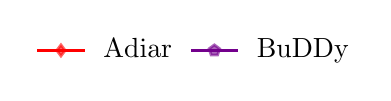
\begin{tikzpicture}
      \begin{customlegend}[
        legend columns=-1,
        legend style={draw=none,column sep=1ex},
        legend entries={
          Adiar,
          BuDDy
        }
        ]
        \addlegendimage{style=plot_adiar}
        \addlegendimage{style=plot_buddy}
      \end{customlegend}
    \end{tikzpicture}

    %\caption{Relational Product for MCC models with a $2^{25}$ state space BDD. Timeouts are marked
    %         as stars.}
  \end{figure}
\end{frame}

% Now, these are of course the two coolest positive highlights. There are two
% caviats that I want to highlight with respect to the relational product:
%
% 1. For this particular operation, our experiments indicate that our approach
%    is not only 4 times slower for the medium instances but 10 times slower.
%
%    But, if you dig into the litterature on BDDs and look a bit deeper into
%    our experiments, there are indications as to where to look for performance
%    improvements.
%
% 2. In the case of transition systems, the size of the BDDs explode quite
%    slowly. Now, that sounds like a good thing. But, for our algorithms this
%    is quite bad, since this is the case where it is several orders of
%    magnitude slower.
%
%    But, the thesis includes ideas for how to get the best of both worlds.
%
% So all in all; these are not only 'issues' but just as much 'opportunities'.
% That's what you call 'Future Work', right?
\blankframe

% ---------------------------------------------------------------------------- %
% Chapter 5:
% - Motivation -> Results
% - Insight
% - Solution

% So, that was the highlight of our algorithmic contributions at the top of
% this timeline. At the bottom, we have several optimisations that have been
% vital to obtain this level of performance.
%
% In many ways, these optimisations are quite similar. I'll get to how later.
% Right now, I'd like to go into Levelised Cuts in more detail as an example.
\againframe{timeline}

% First, let us take a look at our initial experiments from back in 2021. On
% the x-axis you have the problem's complexity while on the y-axis you have the
% time spent by both algorithms.
%
% First of all, our algorithm can compute on much larger BDDs - far beyond what
% is possible by BuDDy's algorithms.
%
% But, you may also notice something quite odd: the running time of our
% implementation seems to always use at least 1 second. This turns out to be
% due the fact, that the external memory priority queues we use has to spend
% time initialising its internal memory.
%
% This in fact means, the more memory you have, the slower our algorithms are!
% This really should not be the case - especially in these smaller cases where
% external memory is not needed. We could just use a simpler priority queue
% that does not have such an overhead.
%
% So, the question is: when can we safely replace the expensive external memory
% priority queue? To this end, we need to know how much stuff needs to be
% stored in this priority queue. That is, we need to get an upper bound on its
% size.
\begin{frame}{Levelised Cuts}
  \begin{figure}
    \centering

    \begin{tikzpicture}
      \begin{axis}[%
        width=0.88\linewidth, height=0.42\linewidth,
        every tick label/.append style={font=\scriptsize},
        % x-axis
        xlabel={Problem Complexity (\# BDD nodes)},
        xmajorgrids=true,
        xmin=12000,
        xmax=300000000000,
        xmode = log,
        % y-axis
        ymin=0.001,
        ymax=1000000,
        ymode=log,
        ytick={0.001,0.01,0.1,1,10,100,1000,10000,100000,1000000},
        ylabel={Time (s)},
        yminorgrids=false,
        ymajorgrids=true,
        grid style={dashed,black!20},
        ]

        \addplot+ [style=plot_buddy]
        table {./data/queens_buddy_time.tex};

        \only<1>{
          \addplot+ [style=plot_adiar]
          table {./data/queens_adiar_time.v1.0.0.tex};
        }
        \only<2>{
          \addplot+ [style=plot_adiar, dashed]
          table {./data/queens_adiar_time.v1.0.0.tex};

          \addplot+ [style=plot_adiar]
          table {./data/queens_adiar_time.v1.2.0.tex};
        }
      \end{axis}
    \end{tikzpicture}

    \begin{tikzpicture}
      \only<1>{
        \begin{customlegend}[
          legend columns=-1,
          legend style={draw=none,column sep=1ex},
          legend entries={BuDDy, Adiar v1.0}
          ]
          \addlegendimage{style=plot_buddy}
          \addlegendimage{style=plot_adiar}
        \end{customlegend}
      }
      \only<2>{
        \begin{customlegend}[
          legend columns=-1,
          legend style={draw=none,column sep=1ex},
          legend entries={BuDDy, Adiar v1.2}
          ]
          \addlegendimage{style=plot_buddy}
          \addlegendimage{style=plot_adiar}
        \end{customlegend}
      }
    \end{tikzpicture}

    \caption{Running Time to solve $N$-\emph{Queens} problems.}
  \end{figure}
\end{frame}

% If we take a closer look at our algorithm, we notice something quite
% interesting as it processes a single level of a BDD:
%
%   It has one (or more) priority queue(s) that contain edges to the nodes it
%   needs to process. It retrieves all in-going edges to a node, processes the
%   node, and then puts back into the priority queue the out-going edges to the
%   nodes’ yet-to-be-resolved children. Then, it goes on to do the same for the
%   next node on this level.
%
%   What you might notice is that the edges in the priority queue always are a
%   cut in the output BDD: a cut between the resolved and the
%   yet-to-be-resolved half.
%
%   So, our previous question about the size of the priority queues can be
%   rephrased as a question about how large this cut could be.
\begin{frame}{Levelised Cuts}
  % \begin{center}
  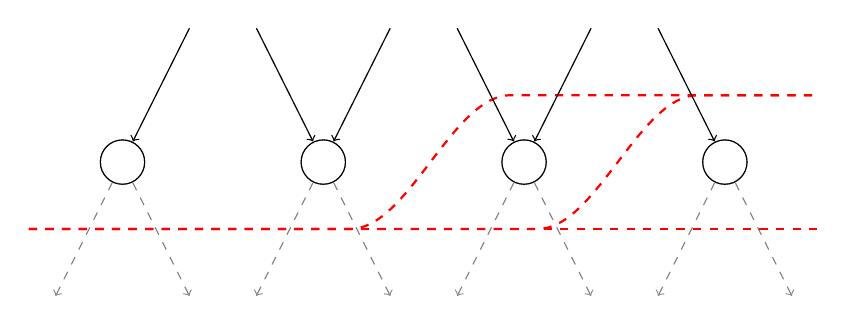
\begin{tikzpicture}[scale=1.7, every node/.style={transform shape}]
    % cut coordinates
    \coordinate (cut_start) at (-0.7,-0.5);
    \coordinate (cut_end_low) at (5.2,-0.5);
    \path (cut_end_low) +(0,1) coordinate (cut_end_high);

    % --------------------------------------------------------------------------
    % before
    \onslide<1> {
      \node[shape = circle, draw = gray] at (0,0)  (0_before) {};
      \draw[gray, dashed, <-] (0_before) -- ++(0.5,1.0);
    }

    % after
    \onslide<2-> {
      \node[shape = circle, draw = black] at (0,0) (0_after) {};
      \draw[black, <-] (0_after) -- ++(0.5,1.0);

      \draw[gray, dashed, ->] (0_after) -- ++(-0.5,-1);
      \draw[gray, dashed, ->] (0_after) -- ++(0.5,-1);
    }

    % --------------------------------------------------------------------------
    % before
    \onslide<-2> {     
      \node[shape = circle, draw = gray] at (1.5,0) (1_before) {};
      \draw[gray, dashed, <-] (1_before) -- ++(-0.5,1.0);
      \draw[gray, dashed, <-] (1_before) -- ++(0.5, 1.0);
    }

    % after
    \onslide<3-> {
      \node[shape = circle, draw = black] at (1.5,0) (1_after) {};
      \draw[black, <-] (1_after) -- ++(-0.5,1.0);
      \draw[black, <-] (1_after) -- ++(0.5, 1.0);

      \draw[gray, dashed, ->] (1_after) -- ++(-0.5,-1);
      \draw[gray, dashed, ->] (1_after) -- ++(0.5,-1);
    }

    % cut
    \onslide<4> {
      \draw[thick, dashed, red]
        (cut_start) -- ++(2.4,0.0) cos ++(0.6,0.5) sin ++(0.6,0.5) -- (cut_end_high)
      ;
    }
    
    % --------------------------------------------------------------------------
    % before
    \onslide<-4> {
      \node[shape = circle, draw = gray] at (3.0,0) (2_before) {};
      \draw[gray, dashed, <-] (2_before) -- ++(-0.5,1.0);
      \draw[gray, dashed, <-] (2_before) -- ++(0.5,1.0);
    }

    % after    
    \onslide<5-> {
      \node[shape = circle, draw = black] at (3.0,0) (2_after) {};
      \draw[black, <-] (2_after) -- ++(-0.5, 1.0);
      \draw[black, <-] (2_after) -- ++(0.5, 1.0);

      \draw[gray, dashed, ->] (2_after) -- ++(-0.5,-1);
      \draw[gray, dashed, ->] (2_after) -- ++(0.5,-1);
    }

    % cut
    \onslide<5> {
      \draw[thick, dashed, red]
        (cut_start) -- ++(3.8,0.0) cos ++(0.6,0.5) sin ++(0.6,0.5) -- (cut_end_high)
      ;
    }

    % --------------------------------------------------------------------------
    % before
    \onslide<-5> {
      \node[shape = circle, draw = gray] at (4.5,0) (3_before) {};
      \draw[gray, dashed, <-] (3_before) -- ++(-0.5,1.0);
    }

    % after
    \onslide<6-> {
      \node[shape = circle, draw = black] at (4.5,0) (3_after) {};
      \draw[black, <-] (3_after) -- ++(-0.5,1.0);      

      \draw[gray, dashed, ->] (3_after) -- ++(-0.5,-1);
      \draw[gray, dashed, ->] (3_after) -- ++(0.5,-1);
    }

    % cut
    \onslide<6> {
      \draw[thick, dashed, red]
        (cut_start) -- (cut_end_low)
      ;
    }
  \end{tikzpicture}
\end{center} with output arcs reversed

  \begin{center}
    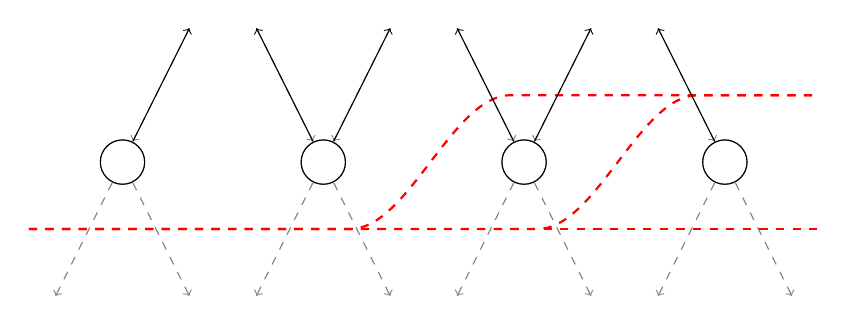
\begin{tikzpicture}[scale=1.7, every node/.style={transform shape}]
      % cut coordinates
      \coordinate (cut_start) at (-0.7,-0.5);
      \coordinate (cut_end_low) at (5.2,-0.5);
      \path (cut_end_low) +(0,1) coordinate (cut_end_high);

      % --------------------------------------------------------------------------
      % before
      \onslide<1> {
        \node[shape = circle, draw = gray] at (0,0)  (0_before) {};
        \draw[gray, dashed, <-] (0_before) -- ++(0.5,1.0);
      }

      % after
      \onslide<2-> {
        \node[shape = circle, draw = black] at (0,0) (0_after) {};
        \draw[black, ->] (0_after) -- ++(0.5,1.0);

        \draw[gray, dashed, ->] (0_after) -- ++(-0.5,-1);
        \draw[gray, dashed, ->] (0_after) -- ++(0.5,-1);
      }

      % --------------------------------------------------------------------------
      % before
      \onslide<-2> {
        \node[shape = circle, draw = gray] at (1.5,0) (1_before) {};
        \draw[gray, dashed, <-] (1_before) -- ++(-0.5,1.0);
        \draw[gray, dashed, <-] (1_before) -- ++(0.5, 1.0);
      }

      % after
      \onslide<3-> {
        \node[shape = circle, draw = black] at (1.5,0) (1_after) {};
        \draw[black, ->] (1_after) -- ++(-0.5,1.0);
        \draw[black, ->] (1_after) -- ++(0.5, 1.0);

        \draw[gray, dashed, ->] (1_after) -- ++(-0.5,-1);
        \draw[gray, dashed, ->] (1_after) -- ++(0.5,-1);
      }

      % cut
      \onslide<4> {
        \draw[thick, dashed, red]
        (cut_start) -- ++(2.4,0.0) cos ++(0.6,0.5) sin ++(0.6,0.5) -- (cut_end_high)
        ;
      }

      % --------------------------------------------------------------------------
      % before
      \onslide<-4> {
        \node[shape = circle, draw = gray] at (3.0,0) (2_before) {};
        \draw[gray, dashed, <-] (2_before) -- ++(-0.5,1.0);
        \draw[gray, dashed, <-] (2_before) -- ++(0.5,1.0);
      }

      % after
      \onslide<5-> {
        \node[shape = circle, draw = black] at (3.0,0) (2_after) {};
        \draw[black, ->] (2_after) -- ++(-0.5, 1.0);
        \draw[black, ->] (2_after) -- ++(0.5, 1.0);

        \draw[gray, dashed, ->] (2_after) -- ++(-0.5,-1);
        \draw[gray, dashed, ->] (2_after) -- ++(0.5,-1);
      }

      % cut
      \onslide<5> {
        \draw[thick, dashed, red]
        (cut_start) -- ++(3.8,0.0) cos ++(0.6,0.5) sin ++(0.6,0.5) -- (cut_end_high)
        ;
      }

      % --------------------------------------------------------------------------
      % before
      \onslide<-5> {
        \node[shape = circle, draw = gray] at (4.5,0) (3_before) {};
        \draw[gray, dashed, <-] (3_before) -- ++(-0.5,1.0);
      }

      % after
      \onslide<6-> {
        \node[shape = circle, draw = black] at (4.5,0) (3_after) {};
        \draw[black, ->] (3_after) -- ++(-0.5,1.0);

        \draw[gray, dashed, ->] (3_after) -- ++(-0.5,-1);
        \draw[gray, dashed, ->] (3_after) -- ++(0.5,-1);
      }

      % cut
      \onslide<6> {
        \draw[thick, dashed, red]
        (cut_start) -- (cut_end_low)
        ;
      }
    \end{tikzpicture}
  \end{center}
\end{frame}

% In fact, this cut has a very particular shape which we can formalise as an
% *i-level cut*: given that every node of a directed acyclic graph is assigned
% some level, we restrict the cut to span at most i levels.
%
% In particular, a 1-level cut is a horizontal cut and a 2-level cut only
% leaves a single level free to move between either side of the cut.
%
% Theorem:
%   Now, if we have the maximum 2-level cuts of two input BDDs, then we can
%   upper bound the output's maximum 2-level cut by their product.
%
%   Since it is cheaper to compute the maximum 1-level cut size, we would want
%   to use that one to bound the 2-level cut if possible. In fact we can,
%   because for BDDs the size of the 2-level cut can at most be three halves
%   larger!
%
% The only thing missing is to compute the cut sizes in the first place...
\begin{frame}{Levelised Cuts}
  \begin{columns}
    \begin{column}[b]{0.55\textwidth}
      \begin{center}
        \textbf{\LARGE \emph{i}-level cut}
      \end{center}

      \begin{tikzpicture}[scale=0.9]
        % levels
\node (Lcal) {\color{orange} $\mathcal{L}$};

\node[below=0.5cm of Lcal] (Lj) {\color{orange} $j$};
\node[below=0.5cm of Lj] (Lj1) {\color{orange} $j+1$};
\node[below=0.5cm of Lj1] (Ldots) {\color{orange} $\vdots$};
\node[below=0.6cm of Ldots] (Lji) {\color{orange} $j+i$};

\draw[dashed, orange]
  ($ (Lj) + (1,0) $) edge ($ (Lj) + (7,0) $)
;

\draw[dashed, orange]
  ($ (Lji) + (1,0) $) edge ($ (Lji) + (7,0) $)
;
    
% nodes
\node[shape = circle, draw = black, fill=white, right=2cm of Lj] (j_1) {};
\node[shape = circle, draw = black, fill=white, right=3cm of Lj] (j_2) {};
\node[shape = circle, draw = black, fill=white, right=5cm of Lj] (j_3) {};

\node[shape = circle, draw = black, fill=white, right=2.5cm of Lj1] (j1_1) {};
\node[shape = circle, draw = black, fill=white, right=4cm of Lj1] (j1_2) {};

\node[right=3.8cm of Ldots] (jdot_1) {$\cdot$};
\node[right=5.3cm of Ldots] (jdot_2) {$\cdot$};
    
\node[shape = circle, draw = black, fill=white, right=1.5cm of Lji] (ji_1) {};
\node[shape = circle, draw = black, fill=white, right=3cm of Lji] (ji_2) {};
\node[shape = circle, draw = black, fill=white, right=5cm of Lji] (ji_3) {};
    
% arcs
\draw[->]
% to level j
  ($ (j_1) + (-0.5,0.5) $) edge (j_1)
  ($ (j_1) + (0.5,0.5) $) edge (j_1)

  ($ (j_2) + (0,0.5) $) edge (j_2)

  ($ (j_3) + (-0.5,0.5) $) edge (j_3)
  ($ (j_3) + (0.5,0.5) $) edge (j_3)
    
% to level j+1
  (j_1) edge (j1_1)
  (j_2) edge (j1_1)
  ($ (j_2) + (1,0.5) $) edge (j1_2)
  (j_3) edge (j1_2)
      
% to levels in between
  (j1_2) edge[bend right=10] (jdot_1)
  (j1_2) edge[bend left=20] (jdot_2)
  (j_3) edge[bend left=15] (jdot_2)
  (j_3) edge[bend left=50] (jdot_2)
      
% to level j+i
  ($ (j_1) + (-0.7,0.5) $) edge[bend right=10] (ji_1)
  (j_1) edge[bend left=5] (ji_1)
  (j_2) edge[bend left=5] (ji_2)
  (jdot_1) edge[bend left=10] (ji_2)
  (jdot_2) edge[bend left=20] (ji_3)
  (jdot_2) edge[bend right=20] (ji_3)

% past level j+i
  (j1_1) edge[bend left=5] ($ (ji_1) + (0.7,-0.5) $)
  (jdot_1) edge[bend right=10] ($ (ji_2) + (1,-0.5) $)
  (ji_1) edge ($ (ji_1) + (-0.5,-0.5) $)
  (ji_1) edge ($ (ji_1) + (0.5,-0.5) $)
  (ji_2) edge ($ (ji_2) + (0,-0.5) $)
  (ji_3) edge ($ (ji_3) + (-0.5,-0.5) $)
  ($ (j_3) + (1,0.5) $) -> ($ (ji_3) + (1,-0.5) $)
;

% cut
\draw[thick, dashed, red]
  ($ (j_1) + (-1.2, -1.5) $) sin
  ($ (j_2) + (-0.2, -0.5) $) cos
  ($ (j_2) + (0.4, -2) $) sin
  ($ (jdot_1) + (0.0, -0.5) $) cos
  ($ (jdot_1) + (0.2, 0) $) --
  ($ (j1_2) + (-0.3, 0) $) sin
  ($ (j1_2) + (0, 0.5) $) cos
  ($ (j1_2) + (0.4, 0) $) sin
  ($ (j1_2) + (1.1, -1.8) $) --
  ($ (j1_2) + (2.2, -1.8) $)
;

      \end{tikzpicture}
    \end{column}
    \begin{column}[b]{0.44\textwidth}
      \onslide<2-> {
        \begin{theorem}
          Given maximum $2$-level cuts size $C_{\phi}$ for BDD $\phi$ and
          $C_{\psi}$ for BDD $\psi$, the maximum $2$-level cut for the BDD
          $\phi \land \psi$ is less than or equal to $C_{\phi} \cdot C_{\psi}$.
        \end{theorem}
      }

      \onslide<3-> {
        \begin{lemma}
          The maximum $2$-level cut for BDD $\phi$ is at most $\tfrac{3}{2}$
          larger than its maximum $1$-level cut.
        \end{lemma}
      }
    \end{column}
  \end{columns}
\end{frame}

% ... luckily, it turns out that we can compute an over-approximation of the
% i-level cuts as part of the Apply and Reduce sweeps I showed you earlier.
%
% By approximating the 1-level cut and multiplying it with three halves, we
% only pay a single 1 percent in running time overhead. The accuracy on the
% size of the priority queue is pretty good.
%
% We can improve the accuracy by computing the 2-level cut directly. But, in
% practice the additional precision is not worth the additional overhead.
\begin{frame}{Levelised Cuts}
  \begin{table}[ht!]
    \centering

    { \LARGE
      \begin{tabular}{lccc}
        &               & +\faIcon{stopwatch}  & \faIcon{ruler}
        \\
        &               & \normalsize Overhead & \normalsize Precision
        \\ \hline
        1-level cut & \quad : \quad & $1.0\%$  & 69.2\%
        \\
        2-level cut & \quad : \quad & $3.3\%$  & 86.3\%
      \end{tabular}
    }
  \end{table}
\end{frame}

% The other optimisation follow a similar theme: we make the algorithm adapt to
% the given BDDs based on some information about its structure that is cheap to
% compute.
%
% That is, we also compute some additional information next to the BDD. This
% information provides us with some guarantees. Based on these, we can change
% the algorithm in subtle - or not so subtle - ways.
\againframe{timeline}

% ---------------------------------------------------------------------------- %
% Take Home Message:
%
% As a result of all this work, I can present you with the *Adiar* BDD package.
% It is (1) open source (2) under the permissive MIT license, (3) it is written
% to be proper production-grade quality with more than 3000 unit tests, and (4)
% has an extensive documentation for its flexible API.
%
% Already now, Adiar is a useful tool for applications where the BDDs grow
% large very quickly.
%
% In the thesis we also sketch the two most pressing future directions for this
% project - specifically we show to fix the slow performance on smaller
% instances and how to change the variable ordering of the BDDs.
%
% And, this work we hopefully are one step closer to verify more complex
% critical system we rely on every day.
\begin{frame}{}

  {\Large \textbf{Adiar}}
  \vspace{1pt} {\hrule width\linewidth}

  \begin{columns}
    \begin{column}[t]{0.45\linewidth}
      \begin{itemize}
      \item[\faIcon{code}]
        \href{http://github.com/ssoelvsten/adiar}{github.com/ssoelvsten/adiar}
      \item[\faIcon{balance-scale}]
        MIT
      \end{itemize}
    \end{column}
    \begin{column}[t]{0.45\linewidth}
      \begin{itemize}
      \item[\faIcon{book}\hspace{2pt}]
        \href{http://ssoelvsten.github.io/adiar}{ssoelvsten.github.io/adiar}
      \item[\faIcon{check}]
        3.462 unit tests
      \end{itemize}
    \end{column}
  \end{columns}

  \bigskip\pause

  {\Large \textbf{Future Work}}
  \vspace{1pt} {\hrule width\linewidth}
  \faStyle{regular}

  \begin{columns}
    \begin{column}[t]{0.45\linewidth}
      \begin{itemize}
      \item[\faIcon{rocket}]
        Small Instances

        \vspace{-10pt}
        \begin{center}
          \begin{tikzpicture}
            \begin{axis}[%
              width=1\linewidth, height=0.6\linewidth,
              every tick label/.append style={font=\tiny},
              % x-axis
              xlabel={\tiny \texttt{Adiar} Running Time (s)},
              xmin=0.01,
              xmax=10000,
              xtick={0.01,0.1,1,10,100,1000,10000},
              xmode=log,
              % y-axis
              ylabel={\tiny \texttt{BuDDy} (Relative)},
              ymin=0.00390625,
              ymax=5.0,
              ytick = {0.00390625,0.015625,0.0625,0.25,1,4},
              yticklabels = {
                ,
                $2^{-6} \times$,
                ,
                $2^{-2} \times$,
                ,
                $2^{2} \times$
              },
              ymode=log,
              % grid
              grid style={dashed,black!12},
              ]

              % data (solved)
              \addplot+ [forget plot, style=dots_buddy, mark options={color=gray, fill=gray, opacity=0.6}]
              table {./data/qbf.buddy.solved.tex};

              % data (timeouts)
              \addplot+ [forget plot, style=x_buddy, mark options={color=gray, fill=gray, opacity=0.6}]
              table {./data/qbf.buddy.timeouts.tex};

              % data (small)
              \addplot+ [forget plot, style=dots_buddy]
              table {./data/qbf.buddy.small.tex};

              % vertical 1s line
              \draw[densely dotted, opacity=0.4] (0,1.0) -- (0,-5.0);
              % vertical 100s line
              \draw[densely dotted, opacity=0.4] (4.6,1.0) -- (4.6,-5.0);

              % 1 line
              \addplot[domain=0.001:100000, samples=8, color=black]
              {1};
            \end{axis}
          \end{tikzpicture}
        \end{center}
      \end{itemize}
    \end{column}
    \begin{column}[t]{0.45\textwidth}
      \begin{itemize}
      \item[\faIcon{sort-alpha-down}]
        Variable Reordering

        \vspace{10pt}
        \begin{center}
          \resizebox{0.8\textwidth}{!}{%
            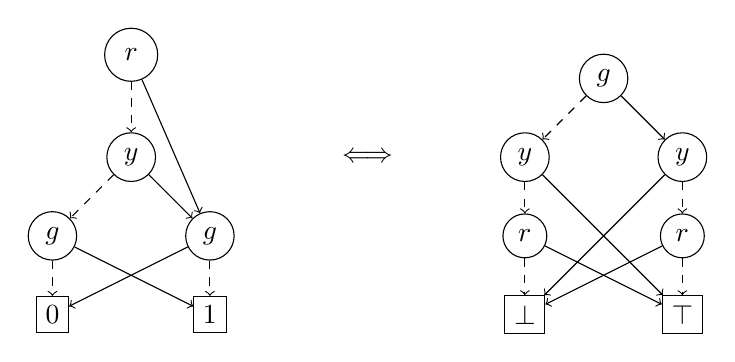
\begin{tikzpicture}
              % Fig 1.4
\node[shape=circle, draw=black, fill=white, inner sep=4.5pt] at (0, 0.3)
(r) {$r$};

\node[shape=circle, draw=black, fill=white] at ( 0, -1)
(y) {$y$};

\node[shape=circle, draw=black, fill=white] at (-1, -2)
(g1) {$g$};

\node[shape=circle, draw=black, fill=white] at ( 1, -2)
(g2) {$g$};

\node[shape=rectangle, draw=black, fill=white] at (-1,-3)
(bot) {$0$};
\node[shape=rectangle, draw=black, fill=white] at ( 1,-3)
(top) {$1$};

\draw[->, dashed]
  (r)  edge (y)
  (y)  edge (g1)
  (g1) edge (bot)
  (g2) edge (top)
;
\draw[->]
  (r)  edge (g2)
  (y)  edge (g2)
  (g1) edge (top)
  (g2) edge (bot)
;

              % iff
              \node[] at (3, -1) {$\iff$};

              % Fig 1.4(b)
              \node[shape=circle, draw=black] at ( 6, 0)
              (g) {$g$};

              \node[shape=circle, draw=black] at ( 5, -1)
              (y1) {$y$};

              \node[shape=circle, draw=black] at ( 7, -1)
              (y2) {$y$};

              \node[shape=circle, draw=black] at ( 5, -2)
              (r1) {$r$};

              \node[shape=circle, draw=black] at ( 7, -2)
              (r2) {$r$};

              \node[shape=rectangle, draw=black] at ( 5,-3)
              (bot) {$\bot$};
              \node[shape=rectangle, draw=black] at ( 7,-3)
              (top) {$\top$};

              \draw[->, dashed]
                (g)  edge (y1)
                (y1) edge (r1)
                (y2) edge (r2)
                (r1) edge (bot)
                (r2) edge (top)
              ;
              \draw[->]
                (g)  edge (y2)
                (y1) edge (top)
                (y2) edge (bot)
                (r1) edge (top)
                (r2) edge (bot)
              ;
            \end{tikzpicture}
          }
        \end{center}
      \end{itemize}
    \end{column}
  \end{columns}
\end{frame}

% ---------------------------------------------------------------------------- %
% Appendix
\blankframe

\begin{frame}[t]{Manual Variable Reordering}

  Consider the \texttt{bdd\_replace}($f$, $\pi$) from \texttt{BuDDy} to compute
  $[x \mapsto \pi(x)]$ on an input with $N$ BDD nodes and $n$ variables and an
  output of $T$ BDD nodes.

  \begin{table}
    \centering
    \begin{tabular}{ll||cc}
      &              & Depth-first
                     & Time-forwarding
      \\ \hline \hline
      \multirow{2}*{Any $\pi$}
      & Time \& I/Os & \multirow{2}*{$\Oh{N + n \cdot T}$}
                     & $\Oh{\sort{T \cdot \sum_{i=1}^n C_{1:f[i]}^{\emptyset}}}$
      \\
      & Space        &
                     & $\Oh{\sort{T \cdot \max_{i}(C_{1:f[i}^{\emptyset})}}$
      \\ \hline
      \multirow{2}*{Exchange}
      & Time \& I/Os & \multirow{2}*{$\Oh{N + T}$}
                     & $\Oh{\sort{N + T}}$
      \\
      & Space        &
                     & $\Oh{N + T}$
      \\ \hline
      \multirow{2}*{Adjacent Swap}
      & Time \& I/Os & \multirow{2}*{$\Oh{N + T}$}
                     & $\Oh{\sort{N + T}}$
      \\
      & Space        &
                     & $\Oh{N + T}$
    \end{tabular}
  \end{table}
\end{frame}

\begin{frame}[t]{Dynamic Variable Reordering}

  We have surveyed current dynamic variable ordering methods to uncover how our
  I/O-efficient manual reordering algorithms can be applied.
  \begin{itemize}
  \item[] \textbf{Metaheuristics:} simulated annealing, genetic and memetic
    algorithms, and swarm intelligence algorithms, via \emph{exchanges} and
    \emph{adjacent swaps}\footnote{Or any \emph{non-monotone} $\pi$ if that
      does not break the memory limits.}.

  \item[] \textbf{Sifting:} Rudell's sifting algorithm, via repeated
    \emph{exchanges}.

  \item[] \textbf{Parallel Sifting:} Rudell's procedure via repeated
    \emph{adjacent swaps}; this is akin to the 2-window algorithm.
  \end{itemize}

  \smallskip

  In terms of space, these I/O-efficient variants are on par with the
  depth-first approach.
\end{frame}

\blankframe

\begin{frame}
  \begin{itemize}
  \item \textbf{Unique Identifier:}

    \small Sorting predicates can be turned into mere 64-bit integer
    comparison.

  \item \textbf{Levelised Priority Queue:}

    \small Defer sorting of level $\ell$ in the priority queue until level
    $\ell$ has to be processed.

  \item \textbf{Equality Checking:}

    \small If BDDs $\phi$ and $\psi$ are created by \texttt{Reduce} then they
    are bit-wise equivalent iff $\phi \equiv \psi$.

  \item \textbf{Levelised Cuts:}

    \small The priority queue's size is at most the maximum cut in the BDD.

  \item \textbf{Levelised Random Access:}

    \small If a BDD's level fits into memory then random access can be used (in
    moderation).

  \item \textbf{Node Table:}

    \small If a BDD is small enough then compute on it with the conventional
    approach.
  \end{itemize}
\end{frame}

\begin{frame}{Unique Identifier}
  \begin{figure}
    \centering

    \begin{subfigure}{0.9\linewidth}
      \centering

      \begin{tikzpicture}
        \input{tikz/uid_null.tex}
      \end{tikzpicture}

      \caption{\texttt{null}.}
    \end{subfigure}

    \begin{subfigure}{0.9\linewidth}
      \centering

      \begin{tikzpicture}
        \fill[black!5!white] (0,0) rectangle ++(5.4,.6);

\draw[black!60!white, pattern=north east lines, pattern color=black!30!white]
(0,0) rectangle ++(0.2,.6)
node[pos=.5]{\small\color{black} $1$};

\draw[black!60!white, pattern=north west lines, pattern color=black!30!white]
(0.2,0) rectangle ++(5,.6)
node[pos=.5]{\small\color{black} \texttt{v}};

\draw[black!60!white, pattern=north east lines, pattern color=black!30!white]
(5.2,0) rectangle ++(0.2,.6)
node[pos=.5]{\small\color{black} \texttt{f}};

      \end{tikzpicture}

      \caption{\texttt{leaf} with value $0$ or $1$.}
    \end{subfigure}

    \begin{subfigure}{0.9\linewidth}
      \centering

      \begin{tikzpicture}
        \fill[black!5!white] (0,0) rectangle ++(5.4,.6);

\draw[black!60!white, pattern=north east lines, pattern color=black!30!white]
(0,0) rectangle ++(0.2,.6)
node[pos=.5]{\small\color{black} $0$};

\draw[black!60!white, pattern=north west lines, pattern color=black!30!white]
(0.2,0) rectangle ++(1.5,.6)
node[pos=.5]{\small\color{black} \texttt{label}};

\draw[black!60!white, pattern=north east lines, pattern color=black!30!white]
(1.7,0) rectangle ++(3.5,.6)
node[pos=.5]{\small\color{black} \texttt{identifier}};

\draw[black!60!white, pattern=north west lines, pattern color=black!30!white]
(5.2,0) rectangle ++(0.2,.6)
node[pos=.5]{\small\color{black} \texttt{f}};

\draw[black!80!white]
(0,0) rectangle ++(5.4,.6);

      \end{tikzpicture}

      \caption{\texttt{node} with label, \texttt{i}, identifier, \texttt{id}, and an
        out-degree index, \texttt{o}.}
    \end{subfigure}
  \end{figure}
\end{frame}

\begin{frame}{Levelised Priority Queue}
    \begin{center}
    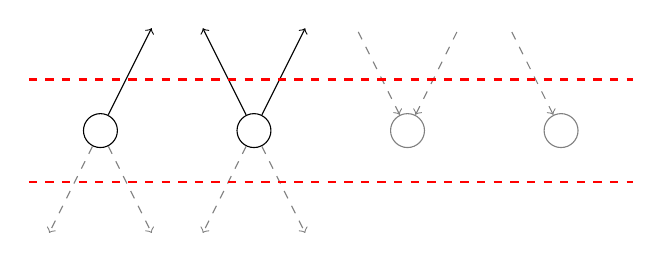
\begin{tikzpicture}[scale=1.3, every node/.style={transform shape}]
      \node[shape = circle, draw = black] at (0,0) (0_after) {};
      \draw[black, ->] (0_after) -- ++(0.5,1.0);

      \draw[gray, dashed, ->] (0_after) -- ++(-0.5,-1);
      \draw[gray, dashed, ->] (0_after) -- ++(0.5,-1);

      \node[shape = circle, draw = black] at (1.5,0) (1_after) {};
      \draw[black, ->] (1_after) -- ++(-0.5,1.0);
      \draw[black, ->] (1_after) -- ++(0.5, 1.0);

      \draw[gray, dashed, ->] (1_after) -- ++(-0.5,-1);
      \draw[gray, dashed, ->] (1_after) -- ++(0.5,-1);

      \node[shape = circle, draw = gray] at (3.0,0) (2_before) {};
      \draw[gray, dashed, <-] (2_before) -- ++(-0.5,1.0);
      \draw[gray, dashed, <-] (2_before) -- ++(0.5,1.0);

      \node[shape = circle, draw = gray] at (4.5,0) (3_before) {};
      \draw[gray, dashed, <-] (3_before) -- ++(-0.5,1.0);

      % --------------------------------------------------------------------------
      \draw[red, dashed, thick] (-0.7, -0.5) -- (5.2, -0.5);
      \draw[red, dashed, thick] (-0.7,  0.5) -- (5.2,  0.5);
    \end{tikzpicture}
  \end{center}

  \begin{columns}
    \begin{column}{0.5\textwidth}
      \textbf{Observation:} When processing level $i$, no new requests for the
      same level are made.

      \bigskip

      \textbf{Optimisation:} Sort bucket of \emph{all} requests for level $i$
      at once with Quicksort ($\sim 2 \times$ faster than a priority queue).
    \end{column}
    \begin{column}{0.4\textwidth}
      \begin{table}
        \centering
        \begin{tabular}{rc}
                           & \faIcon{stopwatch}
          \\
                           & \small Improvement (\%)
          \\ \hline
          Queens (14)      & 25.3
          \\
          Tic-Tac-Toe (22) & 37.0
        \end{tabular}
      \end{table}
    \end{column}
  \end{columns}
\end{frame}

\begin{frame}{Equality Checking}
  \begin{columns}
    \begin{column}{0.6\textwidth}
      \textbf{$\Oh{\sort{N^2}}$}: compute $f \leftrightarrow g$ and check
      whether it is the $1$ BDD.

      \bigskip

      \textbf{$\Oh{\sort{N}}$}: Fail-fast during a product construction if
      more than $N_{f,i}$ ($N_{g,i}$) pairs of nodes are checked on level $i$.

      \bigskip

      \textbf{$2 \cdot \scan{N}$}: Fail-fast during a linear scan of both BDDs
      bit-by-bit.
    \end{column}
    \begin{column}{0.4\textwidth}
      \begin{table}
        \centering
        \begin{tabular}{rc}
                             & \faIcon{stopwatch}
          \\
                             & \small Time (s)
          \\ \hline
          $\Oh{\sort{N^2}}$  & 0.38
          \\
          $\Oh{\sort{N}}$    & 0.058
          \\
          $2 \cdot \scan{N}$ & 0.006
        \end{tabular}

        \caption{Checking the (EPFL Benchmark) \emph{voter} circuit's single output
          gate ($\abs{N_f} = \abs{N_g} = 5.76~\text{MiB}$).}
      \end{table}
    \end{column}
  \end{columns}
\end{frame}

\begin{frame}{Levelised Random Access}
  \begin{columns}
    \begin{column}{0.5\textwidth}
      \centering

      \begin{tikzpicture}
        \node[shape = circle, draw = black] (s) {\large $x_i$};

        % First node
        \node[shape = circle, draw = black, below left=3 and 2 of s] (t) {\large $x_j$};

        \node[below left  = 0.5 and 0.2 of t] (alpha) {$\alpha$};
        \node[below right = 0.5 and 0.2 of t] (beta)  {$\beta$};

        \draw[->, dashed] (t) edge (alpha);
        \draw[->] (t) edge (beta);

        \onslide<2->{
          \draw[->, densely dotted, thick](s) edge[bend right] node[above left] {$\texttt{PQ}_{1}$} (t);
        }

        % Second node
        \onslide<3-> {
          \node[below=3 of s] {$\cdots$};

          \node[shape = circle, draw = black, below right=3 and 2 of s] (u) {\large $x_j$};

          \node[below left  = 0.5 and 0.2 of u] (gamma) {$\gamma$};
          \node[below right = 0.5 and 0.2 of u] (delta) {$\delta$};

          \draw[->, dashed] (u) edge (gamma);
          \draw[->] (u) edge (delta);
        }

        \onslide<4> {
          \draw[->, densely dotted, thick] (t) edge[bend left] node[above] {$\texttt{PQ}_{2}$} (u);
        }
        \onslide<5-> {
          \draw[->, lightgray, densely dotted, thick] (t) edge[bend left] node[above] {$\texttt{PQ}_{2}$} (u);

          \node[red, opacity=0.8] at (-0.07,-2.6) {\fontsize{42}{0} \faIcon{times}};
        }
      \end{tikzpicture}
    \end{column}
    \begin{column}{0.5\textwidth}
      \centering

      \begin{tikzpicture}
        \begin{axis}[%
          width=0.96\linewidth, height=0.5\linewidth,
          every tick label/.append style={font=\scriptsize},
          % x-axis
          xlabel={\# Queens},
          xtick={14,15,16},
          xmajorgrids=true,
          xmin=13.5,
          xmax=16.5,
          % y-axis
          ymin=100,
          ymax=100000,
          ymode=log,
          ytick={10,100,1000,10000,100000,1000000},
          ylabel={Time (s)},
          yminorgrids=false,
          ymajorgrids=true,
          grid style={dashed,black!20},
          ]

          \colorlet{adiar}{red}
          \colorlet{cudd}{orange}

          \tikzstyle{plot_adiar}=[color=adiar, mark=diamond*, mark size=2pt, line width=1pt,
          mark options={color=adiar, fill=adiar, opacity=0.6}]
          \tikzstyle{plot_cudd}=[color=cudd, mark=triangle*, mark size=2pt, line width=1pt,
          mark options={color=cudd, fill=cudd, opacity=0.6}]


          \addplot [style=plot_cudd] coordinates {
            (13, 52.881)
            (14, 316.093)
            (15, 2687.585)
          };

          \only<-4> {
            \addplot [style=plot_adiar] coordinates {
              (13, 82.715)
              (14, 502.855)
              (15, 3336.591)
              (16, 23127.559)
              (17, 196813.872)
            };
          }

          \only<5> {
            \addplot [style=plot_adiar] coordinates {
              (13, 71.277)
              (14, 434.766)
              (15, 2855.766)
              (16, 19400.135)
              (17, 202684.356)
            };
          }
        \end{axis}
      \end{tikzpicture}

      \smallskip

      {
        \small
        \begin{tabular}[b]{cll c c}
                                       &       &                             &   & \faIcon{stopwatch}
          \\ \hline
          {\color{orange} $\triangle$} & CUDD  & v3.0                        & : & 44.8 min%
          \\ \hline
          {\color{red} $\diamond$}     & Adiar & v1.0                        & : & 66.7 min%
          \\
                                       & \multicolumn{2}{l}{+ cuts}          & : & 56.8 min%
          \onslide<5> {
          \\
                                       & \multicolumn{2}{l}{+ random access} & : & 47.2 min}%
        \end{tabular}
      }

      \medskip
      {\footnotesize Counting solutions for the N-Queens Problem.}
    \end{column}
  \end{columns}
\end{frame}

\begin{frame}{Node Table}
  \begin{center}
    \begin{tikzpicture}
      % Boxes
      \draw (0,0) rectangle ++(2,1)
      node[pos=.5]{{\small \texttt{Apply}}{\tiny\it (I/O)}};
      \draw (4,1) rectangle ++(2,1)
      node[pos=.5]{{\small \texttt{Reduce}}{\tiny\it (file)}};
      \draw (4,-1) rectangle ++(2,1)
      node[pos=.5]{{\small \texttt{Reduce}}{\tiny\it (table)}};

      \draw (0,-2) rectangle ++(2,1)
      node[pos=.5]{{\small \texttt{Apply}}{\tiny\it (rec)}};

      % Diamonds
      \node[diamond, draw, inner sep=0.5] (d1) at (-1,-0.5) {\scriptsize $\mathcal{H}_1$};
      \node[diamond, draw, inner sep=0.5] (d2) at ( 3, 0.5) {\scriptsize $\mathcal{H}_2$};

      % Arcs (first decision)
      \draw[->] (-2.5, 0) -- ++(0.4,0) -- ++(0,-0.5) -- (d1);
      \node at  (-2.8, 0) {$f$};
      \draw[->] (-2.5,-1) -- ++(0.4,0) -- ++(0, 0.5) -- (d1);
      \node at  (-2.8,-1) {$g$};

      \draw[<-] ( 0,-1.5) -- ++(-1,0) -- (d1);
      \draw[<-] ( 0, 0.5) -- ++(-1,0) -- (d1);

      % Arcs (second decision)
      \draw[dashed, ->] ( 2, 0.5) -- (d2);

      \draw[dashed, <-] ( 4,-0.5) -- ++(-1,0) -- (d2);
      \draw[dashed, <-] ( 4, 1.5) -- ++(-1,0) -- (d2);

      % Arcs (outputs)
      \draw[->] (6,1.5) -- ++(0.5,0)
      node[pos=3.5]{$f \odot g$ on disk};

      \draw[-] (5,-1) -- ++(0,-0.5);

      \draw[->] (2,-1.5) -- ++(4.5,0)
      node[pos=1.3]{$f \odot g$ in table};
    \end{tikzpicture}
  \end{center}
\end{frame}

\end{document}